
\documentclass[a4paper,12pt]{report}
% arara: pdflatex: { draft: true }
% arara: makeglossaries
% arara: pdflatex: { synctex: true }
% arara: pdflatex: { synctex: true }
% add makeIndex:makeIndex  makeindex %.nlo -s nomencl.ist -o %.nls to commands when running in
\usepackage[square,sort,comma,numbers]{natbib}
\renewcommand{\bibname}{References}
\usepackage[a4paper,bindingoffset=0.2in,left=1in,right=1in,top=1in,bottom=1in,%
footskip=.25in]{geometry}
\bibliographystyle{unsrtnat}

\setcitestyle{authoryear,open={(},close={)}}
\usepackage[utf8]{inputenc}
\usepackage{epsfig}
\usepackage{latexsym}
\usepackage[hidelinks]{hyperref}
\usepackage{graphicx}
\usepackage{subcaption}
\usepackage{amssymb}

\usepackage{tikz}
\usetikzlibrary{shapes.geometric,arrows,positioning,chains}
\newcommand*{\h}{\hspace{5pt}}% for indentation
\newcommand*{\hh}{\h\h}% double indentation


\usepackage[font=scriptsize,labelfont=bf,format=plain,justification=raggedright, singlelinecheck=false]{caption}
\captionsetup[figure, table]{font=scriptsize,labelfont=bf,format=plain,justification=raggedright, singlelinecheck=false}

\usepackage{titlesec}
\titleformat{\chapter}[display]{\bfseries\centering}{\huge Chapter \thechapter}{1em}{\Huge}
%Load nomenclature and glossary files
\usepackage[nottoc]{tocbibind}
\usepackage[intoc]{nomencl}
  \renewcommand{\nomlabel}[1]{#1 \dotfill}

\makenomenclature
\renewcommand{\nomname}{List of Abbreviations}
\usepackage{mathtools}
\usepackage{pdfpages}

\usepackage[page,toc,titletoc,title]{appendix}
%\usepackage{refcheck}

\usepackage{datetime}

\newdateformat{monthyeardate}{%
    \monthname[\THEMONTH], \THEYEAR}

\DeclareGraphicsExtensions{.pdf,.png,.jpg}
\captionsetup{justification=centering,margin=2cm}


\begin{document}


    \title{Develop New Transformer Architecture For \\ Question and Answering}

    \author{Nirbhay P. Tandon\\ Master's of Science in Data Science\\Liverpool John Moore's University}

    \date{\vfill \monthyeardate\today}
    \maketitle


    \cleardoublepage% \clearpage
    \pagenumbering{roman}
    \tableofcontents
    \newpage
    \listoffigures
    \listoftables
    %Nomenclature

\nomenclature{RNNs}{Recurrent Neural Networks}
\nomenclature{LSTMs}{Long Short-Term Memory Architectures}
\nomenclature{NLP}{Natural Language Processing}
\nomenclature{NLU}{Natural Language Understanding}
\nomenclature{RACE}{ReAding Comprehension Dataset From Examinations}
\nomenclature{MCTest}{Machine Comprehension of Text}
\nomenclature{QASENT}{A challenge dataset for open-domain question answering}
\nomenclature{BPPTs}{Back-Propagation Through Time}
\nomenclature{SQuAD}{Stanford Question Answering Dataset}
\nomenclature{CEC}{Constant Error Carousel}
\nomenclature{BERT}{Bidirectional Encoder Representations from Transformers}
\nomenclature{RoBERTa}{Robustly Optimized BERT}
\nomenclature{ALBERT}{A LITE BERT}
\nomenclature{DistilBERT}{Distilled Version of BERT}
\nomenclature{QnA}{Question and Answering}
\nomenclature{BiLSTM}{Bidirectional LSTM}
\nomenclature{SuBiLSTM}{Suffix Bidirectional LSTM}
\nomenclature{CNNs}{Convolutional Neural Networks}
\nomenclature{EM}{Exact Match}
\nomenclature{Ans-Ptr}{Answer-Pointer layer}
\nomenclature{GloVe}{Global Vectors for Word Representation}
\nomenclature{BLEU}{Bilingual Evaluation Understudy}
\nomenclature{WMT}{Workshop on Statistical Machine Translation}
\nomenclature{GPUs}{Graphical Processing Units}
\nomenclature{FFN}{Feed Forward Network(s)}
\nomenclature{MLM}{Masked Language Model}
    \printnomenclature[1in]
	\begin{abstract}
		Attention-based Transformer architectures have become the norm of current Natural Language Processing applications. Google began this trend back in 2017 with their paper \textit{Attention Is All You Need}, by introducing the Transformer architecture that works solely on attention mechanisms. The purpose of this work will be to introduce a variation of the Transformer architecture, \textit{BOLT} or BERT Optimized LSTM Transformer. BOLT is an attempt at combining LSTM based Pointer networks along with a Bidirectional Transformer variant to produce another lighter model specifically for the use of Question Answering. Compare and contrast its performance against other architectures such as RoBerta, DistilBERT and ALBERT using the SQuAD 2.0 Dataset. Through this research it is shown that BOLT is at par with current state of the art architectures and that by combining an LSTM with a Transformer can actually yield slightly better results when correctly optimized.

	\end{abstract}
    \cleardoublepage% \clearpage
    \pagenumbering{arabic}
    \chapter{Introduction}\label{c1introduction}

    One of the most philosophical questions that anyone can encounter is \textit{``Can an answer exist without a question?"}. While that question exists to be solved by philosophers and thinkers, we shall aim to address the \textit{answer} that can be provided to a question in terms of the context that has been asked. While the field of Natural Language Processing(NLP) is vast and many unexplored areas exist, in this thesis the focus is entirely on developing a novel architecture that provides \textit{highly contextual and relevant answers} to the questions asked of it.

        \section{Background Of The Study}\label{c11}
		    The earliest examples of Question-Answering(QA) systems can be traced back to 1961, in the form of BASEBALL,\citep{green1961baseball}, a system developed by Bert F. Green and team to answer basic questions posed using punch cards in ordinary English language about stored data on baseball games. The team implemented a dictionary structure to allow for answers to be looked up and printed. For example, the system could answer very direct questions such as: ``Where did each team play on July 7?".
		    A highly impressive feat for the early days of neural networks in the 1960s, the work done by Green paved the way for systems like LUNAR,\citep{lunar}, answered geological questions for the rocks brought back from the Apollo moon missions. LUNAR, which was first presented in 1971, had an astounding 90\% accuracy rate for questions that were asked by people who didn't know how the system worked!
		    Question-Answering based systems have gained a lot of popularity, especially in the form of ``chatbots''. These systems depend highly on contextual understanding of the input, the training corpus and the question asked. They use this knowledge to output an answer that can help the user with whatever their query is. Recurrent neural networks and architectures based on them, have been able to provide great advancements in the field of Question-answering and chatbots in general. However, there is a behaviour of over-fitting and a lack of contextual understanding of the question. This, coupled with long training times and extremely complex mathematical model designs, have often kept the field of Natural Language Processing slightly obscured from the masses.

		    The task of Question-Answering is a machine comprehension problem. On digging deeper, once can classify it as a sequential problem too. One might wonder how it is a sequential problem? The answer to that is simple, traditionally QA systems work by ``sequentially reading" the input and producing an output based on what they understand semantically or contextually.
		    In a more mathematical context, we can say that the problem we face is of \textit{answer selection} and not \textit{answer provision}. Through numerous studies that have been done, some of which we shall look into detail in chapter \ref{c2litrev}, we see that the problem is not how to provide an answer to a question, it is if the answer provided is the correct one or not in the \textit{context} in which the question has been posed.

		    The research presented forth here is aimed at proposing a new variation to an already successful architecture in the field of NLP, namely \textit{Transformers}, created by the team at Google \citep{atayl}. A critically assessed attempt is made at combining state of the art approaches that have been treated as separate elements so far and to show that the proposed improvements are at par, if not better than the current approach.

		    A Transformer is a form of transduction model that relies solely on self-attention to figure out how to represent its inputs and outputs. It does so without the use of any sequence aligned recurrent neural networks(RNNs) or convolutions.

            The area of Natural language Processing has taken significant leaps in the last two decades. Work done towards improving the ability of machine learning models to first recognize words, then sentences, followed by contextual understanding has led to several interesting and novel approaches in the field. From early on neural networks to creating Long Short-Term Memory architectures \citep{lstmoriginal} by Sepp Hochreiter and Jurgen Schmidhuber in the mid-'90s that resolved the vanishing gradient problem of classical neural networks, we have come a long way.

           The latest advancements in this field come from Google's research lab in the form of \textit{Transformers}. This is studied in a bit more detail later in \ref{c2litrev}. However, no model can be successful without a good dataset to train on. This is where the SQuAD 2.0 dataset \citep{dataset} comes in. This dataset is what forces the machine learning models to do contextual understanding. One might even say that it forces the models to ``think'' for themselves before answering a task.


        \section{Aims And Objectives}\label{12}
        	The main aim of this research is to propose an improvement to the transformer architecture that can perform better at Q\&A using the SQuAD 2.0 dataset. This shall require understanding the nuances of various Transformer-type architectures like ALBERT \citep{albert}, RoBerta \citep{roberta} and DistilBERT \citep{distil} which are variations of the BERT \citep{bert} architecture.

        	To achieve the main aim of this research it  is important to first outline a few steps that will be taken:
        \begin{enumerate}
        	\item Obtain SQuAD2.0 dataset and prepare it for training
        	\item Implement the existing models such as ALBERT, RoBerta and DistilBERT that are available via libraries such as HuggingFace \citep{hfTransformers} and PyTorch  on the dataset
        	\item Obtain F1, Exact Match(EM), Training Loss and Validation Loss scores for existing models to treat them as our benchmark values
        	\item Identify drawbacks of the current architectures
        	\item Design our architecture and evaluate its performance against the provided benchmark scores
        	\item Fine-tune the architecture, re-evaluate and report improvements
        	\item Compare the results of our Transformer model with the benchmark scores.
        \end{enumerate}

        \section{Scope Of The Study}\label{13}

        This research work is entirely focused on the area of Question-Answering based networks. This focus helps in significantly narrowing down the scope and critically assessing the problem that needs to be solved. The practical applications of the field of QA are endless. From chatbots to QA systems on domain-specific knowledge or conversational applications for voice assistants, a light, robust, highly accurate Transformer based architecture can help ease the daily lives of millions of users.

        \section{Significance Of The Study}\label{14}

        The current state of the art systems, some of which have been highlighted in section \ref{c11}, suffer from various drawbacks and even the best models have only been able to achieve an EM score of 90.871 with an F1 score of 93.183 on the SQuAD 2.0 leaderboard \citep{squad}. Current models such as ALBERT and DistilBERT are highly useful, however, they aren't scalable entirely for QA applications. A narrowed focus on the specific field of Question-Answering can help eliminate certain issues with the current models such as contextual uderstanding and being able to get correct responses to questions.

        \section{Structure Of The Study}\label{15}

        This report is divided into 6 main parts, each chapter is further broken down into sections and subsections to localize the reference and use it further in the global context of this research.

        In chapter \ref{c1introduction}, an introduction to the concept of Question-Answering, a brief look at the problem, motivation, scope of this research and its significance have been provided. Chapter \ref{c1introduction} lays the basis of the problem, takes the reader briefly back in time to where QA systems first started and how they have advanced today.

        Chapter \ref{c2litrev}, looks in detail at the background studies that have been briefly mentioned in section \ref{c11}. In this chapter critical analysis is conducted how some of the work that has been selected is relevant to what this research aims to highlight, it helps us understand the merits and shortcomings of current state of the art approaches. Detailed analysis of Long Short-Term Memory(LSTM) and Transformer architectures is written, with special attention to applications in the field of Question Answering. There is particular focus on the advancements and applications of existing architectures as well as acknowledgement of why LSTMs reigned supreme for almost 2 decades. Transformers provide a unique opportunity to perform highly accurate predictive tasks in NLP. The most key advances to both LSTMs and Transformers are their bi-directional applications which are also discussed. Finally, this chapter ends with a summary of the approaches and highlights certain drawbacks. These drawbacks are discussed in more detail in \ref{c4}.

        Next, chapter \ref{c3researchmeth} proposes the research methods that have been implemented. It explains the various metrics that have been used and why they were chosen, specifically highlighting why Accuracy isn't a good measure for creating a successful model and highlighting the use of Precision, Recall and F1 as useful metrics for the experiments conducted in this particular thesis, Exact Match scores are also introduced and discussed in this chapter. The chapter ends with a research flow diagram describing the processes followed for the experiments and application stages of various methods in a visual manner.


        In chapter \ref{c4} the proposed architecture is discussed along with drawbacks of current architectures. The chapter also describes ways in which the proposed architecture can be refined.

        Finally, in chapters \ref{c5} and \ref{c6} the results of the models are discussed while comparing them to current architectures and their benchmarks. The outcomes and various recommendations are outlined that can help improve the work presented in this thesis further.

        Appendix \ref{cgc} is where the reader can refer to the Gantt chart for the thesis work done.

    \chapter{Literature Review}\label{c2litrev}

    To be able to effectively deliver on the aims and objectives we have defined in Section \ref{12}, we must first critically analyse the work that has been done in the field of NLP and, in particular, the field of Question-Answering based networks. In this section, we will critically analyse a few key model architectures and how we reached Transformers, which form the base of our proposed architecture.



        \section{Long Short-Term Memory}\label{22}

            In 1997 \citep{lstmoriginal} introduced to the world a gradient descent based model in the form of Long Short-Term Memory. They set out to solve the problem of the vanishing gradient which was often seen in ``Back-Propagation Through Time"(BPPTs) based neural networks. Extensive studies done on this, some by Hochreiter himself, showed that the problem of vanishing gradients is a real one. It was also seen that in case of BPTTs, the error back-flow mechanisms would either blow up or also suffer from vanishing gradients leading to either oscillating weights or learning to bridge long time gaps would not work. To remediate this, \citep{lstmoriginal} introduced the concept of a \textit{constant} error flow through the internal states of special units.

            Their paper, Long Short-Term Memory, \citep{lstmoriginal}, highlights that the work previously done using various gradient-descent variants, time-delays, time constants, use of higher order units to influence connections when the network receives conflicting error signals, Kalman filters, Second order nets etc. still suffer from some of the same problems that we have earlier. In the case of Ring's approach \citep{lstmRing}, the network can be really fast but also suffers from memory constraints and lack of generalization. This happens because to bridge $ n $ time lags, the model adds $ n $ additional units.

            It is essential for us to understand how LSTMs function as it forms the basis of Transformers to exist. Hochreiter and Scmidhuber designed a \textit{memory cell} that  allows for a constant error flow. This is achieved by introducing \textit{constant error carousel}(CEC), a multiplicative input gate unit and a multiplicative output gate unit. These \textit{multiplicative} units help shield the contents of the memory cell from irrelevant inputs. The CEC, input and output gates together form the \textit{memory cell}, as seen in Fig. \ref{lstmCEC}.
           	\begin{figure}[h!]
      				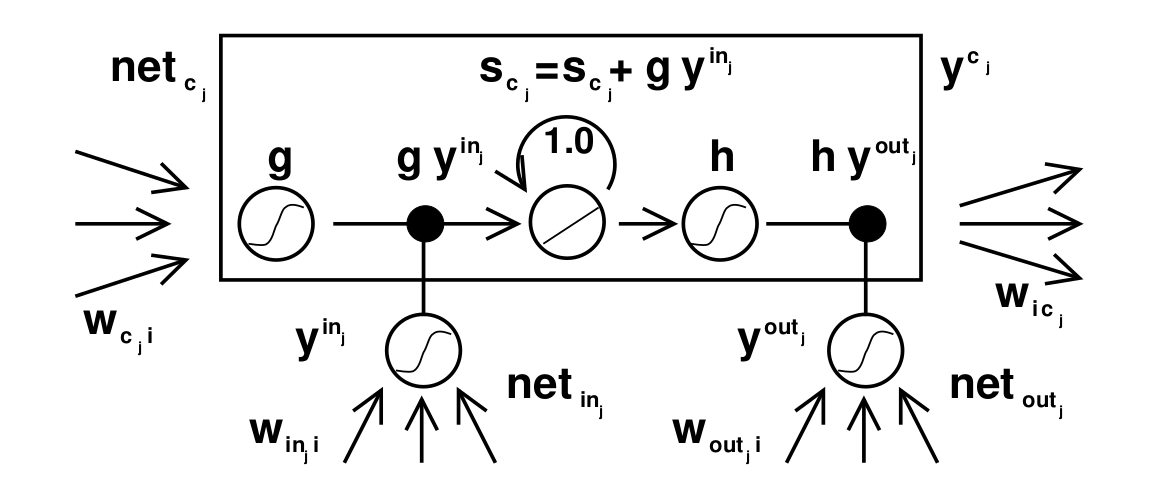
\includegraphics[scale=0.35]{../images/lstm-memorycell.png}
      				\caption{LSTM Memory cell with a Constant Error Carousel having fixed weight 1.0, \citep{lstmoriginal}}\label{lstmCEC}
             \end{figure}
            The central feature for LSTM's memory cell is the CEC. The self-recurrent connection, where weight is 1.0, is what helps create a time-delayed feedback loop by 1.

            The CEC uses gate units to circumvent the issue with conflicting weights in the input and output layers. The input layer has control over when to use and when to override the information in the CEC but has no control over the error signals that are in the memory cell. The output gate, however, uses a feedback mechanism to assess when to superimpose different error signals. It also falls on the output gate to \textit{learn} which errors to trap in the CEC by appropriately scaling them. The gates have to learn when to release and trap errors therefore controlling the access to the CEC, helping maintain constant error flow. To mathematically understand the memory cell from fig. \ref{lstmCEC}, Schmidhuber and Hochreiter proposed the following set of equations \ref{eq1} - \ref{eq3}. More details on this can be found by referring to the appendix section A.1 in \citep{lstmoriginal}.
            \begin{equation}\label{eq1}
                y^{{out }_{j}}(t)=f_{ {out }_{j}}\left( { net }_{ {out }_{j}}(t)\right) ; y^{i n_{j}}(t)=f_{i n_{j}}\left( { net }_{i n_{j}}(t)\right)
            \end{equation}
	        where
            \begin{equation}\label{eq2}
                net_{out_{j}}(t)=\sum_{u} w_{out_{j} u} y^{u}(t-1)
            \end{equation}
            and
            \begin{equation}\label{eq3}
                            net_{in_{j}}(t)=\sum_{u} w_{in_{j} u} y^{u}(t-1)
            \end{equation}
            A generalised form of this equation can be represented as:
            \begin{equation}\label{eq4}
                            net_{c_{j}}(t)=\sum_{u} w_{c_{j} u} y^{u}(t-1)
            \end{equation}
            At time $ t $, $ c_{j} $'s output $ y^{c_{j}}(t) $ is computed as:
            \begin{equation}\label{eq5}
                y^{c_{j}}(t) = y^{out_{j}}(t)h(s_{c_{j}}(t)),
            \end{equation}
            where the ``internal state'' $ s_{c_j}(t) $ is:
            \begin{equation}\label{eq6}
                s_{c_{j}}(0)=0, s_{c_{j}}(t)=s_{c_{j}}(t-1)+y^{i n_{j}}(t) g\left( { net }_{c_{j}}(t)\right) \textrm{for } t>0
            \end{equation}
            Where $ u $ may stand for input, output or gate units, memory cells or even conventional hidden units, if they are being used.

            In fig. \ref{lstmNetwork}, we see the internal workings of how an LSTM network could look like.
            \begin{figure}[!h]
	           \centering
               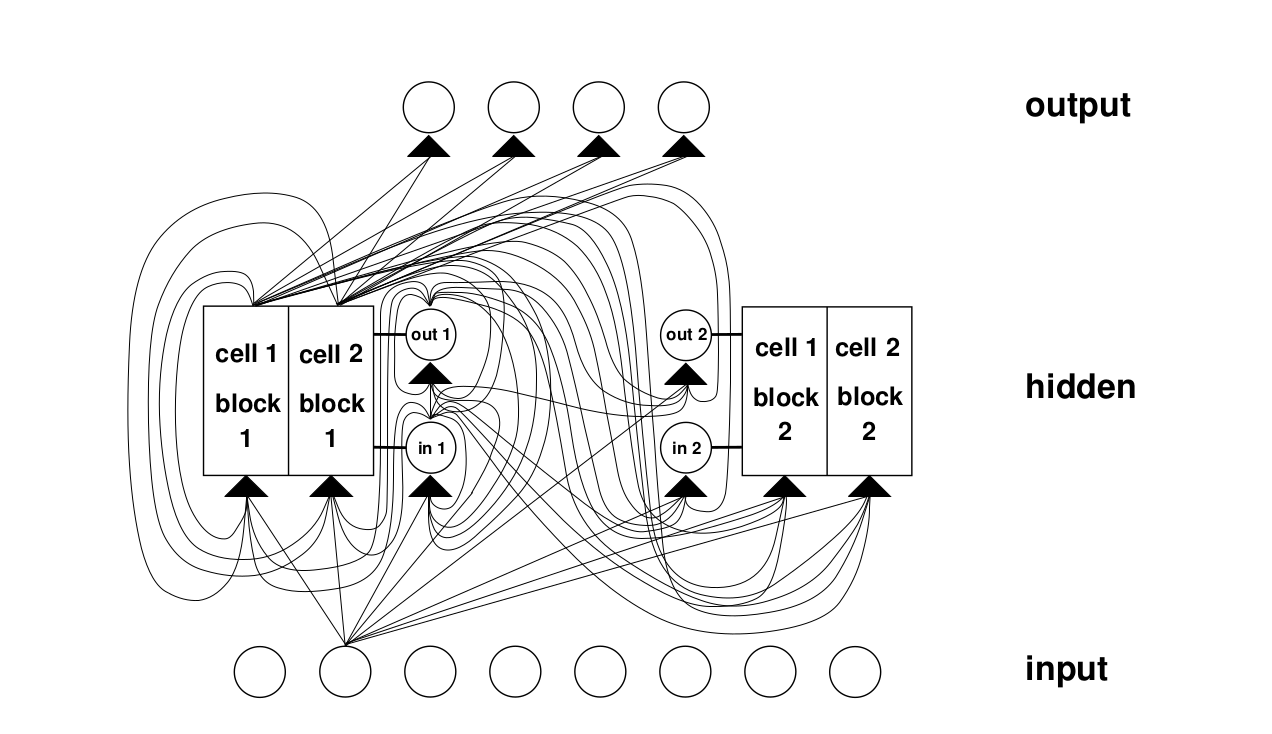
\includegraphics[scale=0.35]{../images/lstm-network.png}
      		   \caption{LSTM network with 8 input cells, 4 output cells and 2 memory cells of block size 2. Here $ in1 \text{and} out1 $ represent the input and output gates and $ cell/block1 $ is the first memory cell. The internal architecture of $ cell/block1 $ is similar to fig. \ref{lstmCEC}. \citep{lstmoriginal}}\label{lstmNetwork}
            \end{figure}

            A series of experiments were performed to prove that LSTMs are indeed ``state-of-the-art" and provide an improvement over then existing RNN based architectures.
            Experiments around temporal order, which is defined as a series of events that happen in a particular order, that were previously unsolved by RNNs, were successfully solved by LSTMs. This was possible because of how LSTMs address time lags vs. how RNNs suffer from vanishing gradients. Details of the analysis and experiments conducted are available in section 5 of the paper ``Long Short-Term Memory" by \citep{lstmoriginal}, with experimental summaries in tables 10 and 11 of the same. Being able to solve for temporal order based problems allowed LSTMs to be capable of solving various real world problems that we will discuss subsequently.
            Temporal orders are key in contextual understanding for NLP based tasks and especially in the case of QA based networks. Let us now look at some advantages and limitations of LSTMs, before moving on to understand how they have been applied in the field of QA.


            \subsubsection{Advantages of LSTMs}
                \begin{itemize}
                    \item LSTMs deal with long time lags by bridging the gaps using constant error flow in the memory cells.
                    \item LSTMs respond well to generalization problems, even if the input sequences are widely separated.
                    \item They work well with a variety of braod range hyper-parameters and don't usually require tuning.
                    \item Their time and weight update complexity is the same as BPTT, ie. $ O(1) $. The advantage for LSTMs however, is that it is local in both space and time.
                \end{itemize}

            \subsubsection{Limitations of LSTMs}
                \begin{itemize}
                    \item LSTMs use memory cells which require an additional input and output unit. This \textit{hidden unit} is replaced by 3 units in an LSTM architecture, compared to 9 in an RNN. A fully connected LSTM will have $ 3^{2} $ connections however.
                    \item LSTMs dont work well when they get the entire input in one go. The architecture is unable to generalize well by random weight guessing in this case.
                    \item They do not have the ability to ``natively" count discrete time steps which might be useful in some applications. This isn't a big issue for the case of QA based problems.
                \end{itemize}

             \subsection{BiLSTMs}\label{c2bilstm}
                  \begin{figure}[!h]
     	           \centering
                    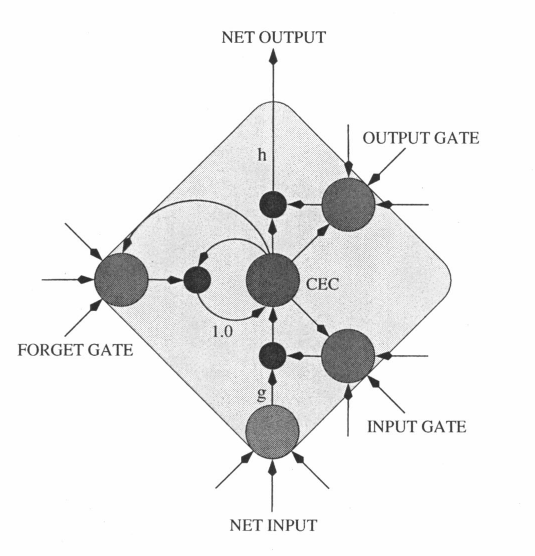
\includegraphics[scale=0.35]{../images/lstm-biLstm.png}
           		   \caption{A memory cell for a biLSTM highlighting a \textit{forget gate}. This forget gate helps in scaling the internal state of a memory cell, for example by resetting the state to 0. We can see that it is different to fig. \ref{lstmCEC}, with the implementation of a connection to the forget gate, while still having an internal weight of 1. \citep{lstmBiLSTM}}\label{lstmBilstm}
                 \end{figure}
            While LSTMs have found various applications across the field of machine and deep learning, QA seems to be one where being able to achieve consistent results of accuracy as well as having an exact match seems to elusive.
            Research carried out at IBM by Tan, Santos and co. looked at approaching this problem by using something called Bidirectional LSTMs or BiLSTM, \citep{lstmBiLSTM}. Introduced by Graves and Schmidhuber in their paper \textit{Framewise Phoneme Classification with Bidirectional LSTM Networks}, the biLSTM implements a \textit{forget gate} as seen in fig. \ref{lstmBilstm}. An advantage of biLSTMs over traditional LSTMs is that you feed the data twice, once from the beginning to the end and then from the end to the beginning. This helps the model contextualize and adjust weights better, therefore creating a more robust model that learns and performs better overall when compared to traditional LSTMs and RNNs.
             \begin{table}[h!]
              \centering
                \begin{tabular}{|c|c|c|c|}
                    \hline
                     & Questions & Answers & Question Word Count \\
                    \hline
                    Train & 12887 & 18540 & 92095 \\
                    \hline
                    Dev & 1000 & 1454& 7158 \\
                    \hline
                    Test1 & 1800 & 2616 & 12893 \\
                    \hline
                    Test2 & 1800 & 2593 & 12905 \\
                    \hline
                \end{tabular}
                \caption{InsuranceQA Corpus Details: Some questions can have multiple answers, therefore the number of answers is greater than the number of questions \citep{lstmInsuranceQA}.}\label{lstmInsuranceQATable}
            \end{table}

            BiLSTMs were introduced as an approach towards phoneme classification for speech recognition applications, however, in their paper ``LSTM-BASED DEEP LEARNING MODELS FOR NON -FACTOID ANSWER SELECTION", \citep{lstmhaighextractive} have shown that extending the biLSTM model 2 different approaches for QA has its advantages. One approach, using a more composite method of using CNNs for representing questions as well as answers. The other, by implementing an \textit{attention mechanism} that helps in generating an answer representation according to the question context.
            Their framework is based on developing a biLSTM model for both questions and answers, applying a connective pooling layer and using a cosine similarity metric to calculate the degree of matching answers. They utilized the InsuranceQA\citep{lstmInsuranceQA} dataset that was created in 2015 and tested primarily on CNN based networks, details of the dataset can be found in table \ref{lstmInsuranceQATable}.

            \begin{figure}
            	\centering
            	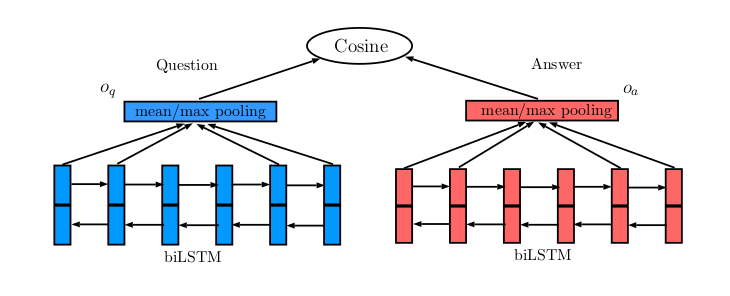
\includegraphics[scale=0.4]{../images/lstm-bilstmhaig.png}
            	\caption{Basic QA-LSTM model depicting biLSTM implementation \citep{lstmhaighextractive}}\label{lstmhaig}
            \end{figure}

            Pooling layers are known to suffer from an incapability to retain local linguistic information. To combat this the team proposed an additional CNN layer on top of the biLSTM layer. Additionally, they added a simple and efficient attention model to help their biLSTM model better distinguish between candidate answers according to the question context. This study is significant in the field of both deep learning based models and for the field of Question-Answering because it requires little or no feature engineering to achieve significant results. In section \ref{23}, how biLSTMs are implemented with Transformers to produce an even better model.

            In their work \citep{lstmhaighextractive} have shown that biLSTMs are capable of capitalizing long-range sequential context information. This is important as it is often seen that the answer is not directly semantically related to the question but more contextually related. Long-range exploitations help the model understand the question more holistically, therefore helping produce a more relevant answer.


		   \begin{figure}
				\centering
				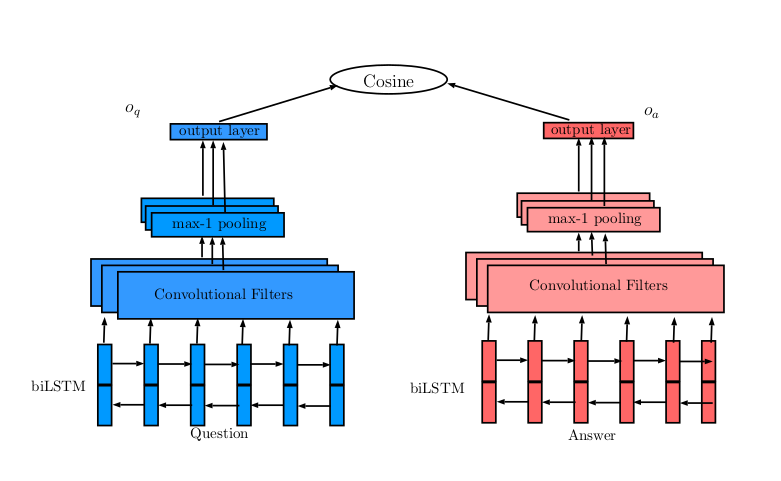
\includegraphics[scale=0.35]{../images/lstm-bilstmhaigcnn.png}
				\caption{QA-LSTM with CNN layer \citep{lstmhaighextractive}}\label{lstmhaigcnn}
			\end{figure}

             BiLSTMs have an advantage over traditional LSTMs in that they utilize both previous and future contextual information by processing the input in both directions, forward and backward. This leads to the generation of two independent sequences of output vectors form LSTMs. The final output is a concatenation  of the outputs from both directions ie. $h_t= \overrightarrow{h_t} || \overleftarrow{h_t} $.
             The \textbf{QA-LSTM} model  proposed by \citep{lstmhaighextractive} can be seen in fig. \ref{lstmhaig}. It can be seen that it generates a distributed representation for both questions(blue) and answers(red) before moving on to perform pooling and cosine similarity operations.
            In fig. \ref{lstmhaigcnn}, it can be seen that the CNN layer has been implemented after the biLSTM layers and before the pooling layers. The pooling layers have been modified to be max-$ k $ pooling layers, similar to standard CNNs.


            The implementation of this convolution layer forces localized interactions between the inputs within a filter size of $ m $. For each window of size $ m $ in biLSTM output vectors ie.
            \begin{equation}
            \textbf{H}_{m}(t)=[\textbf{h}(t), \textbf{h(t+1)},...,\textbf{h}(t+m-1)]
            \end{equation}
            where $ t $ is a time step and the convolution filter will generate one value as follows
            \begin{equation}
                o_{F}(t) = tanh \bigg[\bigg(\sum_{i=0}^{m-1}\textbf{h}(t+i)^{T}\textbf{F}(i)\bigg)+b\bigg]
            \end{equation}

            Using $ k $-MaxPooling,\citep{lstmhaighextractive} emphasized that a maximum of $ k $ values will be kept  for one filter, thereby indicating the highest degree that a filter matches the input sequence. To end this approach, there are $ N $ parallel filters, with different parameter initialization which provide the CNN layer with $ N $-dimension output vectors. This produces two output vectors of dimension $ kN $ for each question and answer.  Their experiments intuitively took $k=1$ as anything greater showed no improvements and it helped emphasize aspects of the answer such that this CNN based hybrid biLSTM could differentiate ground truths and incorrect answers efficiently.

            The second approach adopted in this paper is actually inspired by another paper \citep{bilstmHerman} where attention based deep LSTM networks were used to enhance the capabilities of reading comprehension in LSTM based models. Here, in \citep{lstmhaighextractive}, a modification has been introduced in the form of attention-based connections along with biLSTM layers as depicted in fig. \ref{lstmhaigattention}.
            \begin{figure}
                \centering
                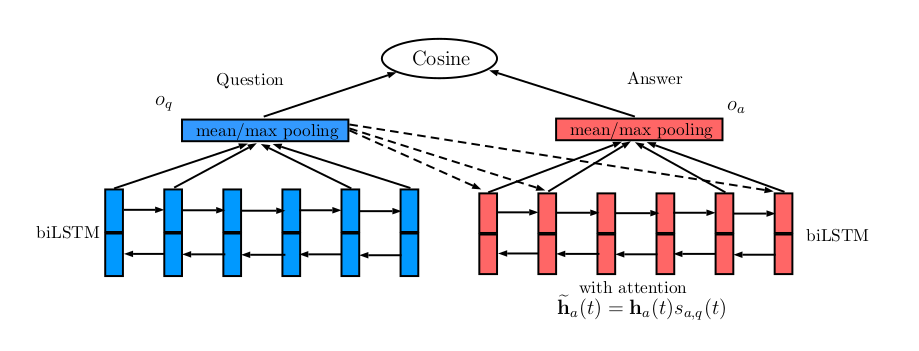
\includegraphics[scale=0.35]{../images/lstm-bilstmhaighattention.png}
                \caption{QA-LSTM with Attention layer \citep{lstmhaighextractive}}\label{lstmhaigattention}
            \end{figure}

            Before conducting a mean/average pooling operation on the output from every biLSTM, the output vectors are multiplied by a softmax weight that is determined by the question embeddings from the biLSTM.
            It was shown that given an output vector from a biLSTM for an answer at time $ t, \textbf{h}_{a}(t)$ and the question embedding, $ o_q $, the updated vector $  \tilde{\textbf{h}_{a}}(t)$ for each answer token
            can be given as:
            \begin{equation}\label{bilstmAttentioneq}
                \textbf{m}_{a,q}(t) = tanh(\textbf{W}_{am}\textbf{h}_{a}(t) + \textbf{W}_{qm}o_{q})
            \end{equation}
            \begin{equation}\label{bilstmattentioneq2}
                s_{a,q}(t) \propto exp(\textbf{w}^{T}_{ms}\textbf{m}_{a,q}(t))
            \end{equation}
            \begin{equation}\label{bilstmattentioneq3}
               \tilde{\textbf{h}_{a}} = \textbf{h}_{a}(t)s_{a,q}(t)
            \end{equation}
            where  $ \textbf{W}_{am}, \textbf{W}_{qm} $ and $ \textbf{w}_ms $ are attention parameters. Attention parameters show somewhat similar behaviour to tf-idf  where some words get more attention or weights associated to them. The main difference being that the attention mechanism adjusts its weights according to question information.

            Critically, this attention based approach from \citep{lstmhaighextractive} emphasizes on attention-driven representations and uses that to calculate the distances between questions and their respective answers. A combination approach with CNNs and attention based connections helps in localizing various internal connections, correctly scaling the errors and reducing unnecessary noise. From eq. \ref{bilstmAttentioneq}-\ref{bilstmattentioneq3}, \citep{lstmhaighextractive} we can mathematically prove how the average distances are computed.
            Experiments conducted on the InsuranceQA dataset showed that the \textit{QA-LSTM/CNN with Attention} model can outperform the taken baseline models, which were based purely on QAs using CNNs.
            \begin{table}
                \begin{tabular}{|l|llll|}
                    \hline & Model & Validation & Test1 & Test2 \\
                    \hline A & QA-LSTM basic-model(head/tail) & $54.0$ & $53.1$ & $51.2$ \\
                    B & QA-LSTM basic-model(avg pooling) & $58.5$ & $58.2$ & $54.0$ \\
                    C & QA-LSTM basic-model(max pooling) & $64.3$ & $63.1$ & $58.0$ \\
                    \hline D & QA-LSTM/CNN(fcount=1000) & $65.5$ & $65.9$ & $62.3$ \\
                    E & QA-LSTM/CNN(fcount=2000) & $64.8$ & $66.8$ & $62.6$ \\
                    F & QA-LSTM/CNN(fcount=4000) & $66.2$ & $64.6$ & $62.2$ \\
                    \hline G & QA-LSTM with attention (max pooling) & $66.5$ & $63.7$ & $60.3$ \\
                    H & QA-LSTM with attention (avg pooling) & $\mathbf{6 8 . 4}$ & $\mathbf{6 8 . 1}$ & $62.2$ \\
                    I & QA-LSTM/CNN (fcount=4000) with attention & $67.2$ & $65.7$ & $\mathbf{6 3 . 3}$ \\
                    \hline
                \end{tabular}
                \caption{Experimental results from \citep{lstmhaighextractive}, highlighting how QA-LSTM with attention outperforms its various modifications}\label{lstmhaigexperiementresults}
            \end{table}

			  An improvement to this approach was done in 2018 by \citep{lstmSubilstm} who proposed \textit{Suffix Bidirectional LSTM} or \textit{SuBiLSTM} adding prefixes and suffixes to the inputs over both directions.  There are a few obvious differences between the biLSTM and SuBiLSTM like the doubling of parameters, increased time complexity which happens over quadratic time for worst case scenarios compared to linear in biLSTMs.
			  \citep{lstmSubilstm} of this paper has shown that despite higher time complexity, there are significant gains in accuracy in text encoding and classification in their experiments, of particular note is the Paraphrase Detection experiment which uses GloVe embeddings and shows an 88.2\% score in the test set, which is marginally higher than other models implemented.
			  The work presented in this thesis will also implement paraphrase detection and GloVe embeddings to potentially improve model performance and answer detection.

			  \subsection{LSTM And Question Answering}\label{c2lstmqa}
             In 2016, the SQuAD dataset \citep{dataset1} was released, that generated quite a buzz in the field of QA based NLP tasks due to its nature of being extremely versatile and crowdsourced.

             Using the SQuAD dataset \citep{lstmhu2016question} developed a match-LSTM \citep{lstmMatch} based model that they showed performed significantly better on the dataset than the work done by \citep{dataset1}. Their work shows that using a match-LSTM approach combined with a Pointer Net model \citep{lstmPointer}, that aids token predictions using only input sequences rather than using any form of large fixed vocabulary, therefore allowing for generation of answers with multiple tokens.

             The approach by \citep{lstmhu2016question} was tw-fold. The first approach implemented as a sequence model and the second as a boundary model, which was further extended with a search function.

             The match-LSTM model architecture consists of:
             \begin{itemize}
             	\item \textbf{LSTM Preprocessing Layer}: As we can see from \ref{lstmMatch}, there are 2 LSTM preporcessing layers. This layer is used to integrate contextual information directly into the representation of how each token in the passage and question is represented. This is based directly on the simple LSTM \citep{lstmoriginal} and not the BiLSTM.
             	\item \textbf{Match-LSTM Layer}: Here, the model treats the question as a premise and the passage as hypothesis. The layer sequentially reads the passage and calculates an attention weight vector $ \vec{\alpha}_{i} \in \mathbb{R}^{Q}$ as:
             	\begin{equation}\label{eqmatchlstm}
             		\begin{aligned}
             			&\overrightarrow{\mathbf{G}}_{i}=\tanh \left(\mathbf{W}^{\mathrm{q}} \mathbf{H}^{\mathrm{q}}+\left(\mathbf{W}^{\mathrm{p}} \mathbf{h}_{i}^{\mathrm{p}}+\mathbf{W}^{\mathrm{r}} \overrightarrow{\mathbf{h}}_{i-1}^{\mathrm{r}}+\mathbf{b}^{\mathrm{p}}\right) \otimes \mathbf{e}_{Q}\right) \\
             			&\vec{\alpha}_{i}=\operatorname{softmax}\left(\mathbf{w}^{\top} \overrightarrow{\mathbf{G}}_{i}+b \otimes \mathbf{e}_{Q}\right)
             		\end{aligned}
             	\end{equation}

			where $\mathbf{W}^{\mathrm{q}}, \mathbf{W}^{\mathrm{p}}, \mathbf{W}^{\mathrm{r}} \in \mathbb{R}^{l \times l}, \mathbf{b}^{\mathrm{p}}, \mathbf{w} \in \mathbb{R}^{l}$ and $b \in \mathbb{R}$ are parameters to be learned, $\overrightarrow{\mathbf{h}}_{i-1}^{\mathrm{r}} \in \mathbb{R}^{l}$ is the hidden vector of the one-directional match-LSTM at position $i-1$, and the outer product $\left(\cdot \otimes \mathbf{e}_{Q}\right)$ produces a matrix or row vector by repeating the vector or scalar on the left for $Q$ times.
			To simply summarise, the above equation \ref{eqmatchlstm} produces  $ \vec{\alpha}_{i,j} $ that gives us the degree of matching between token $ i $ in the passage with token $ j $ in the question. This is the forward pass representation of the mathc-LSTM, the backward pass, which generates encodings for each token in the passage is given by:
			\begin{equation}\label{eqmatchlstmreverse}
				\begin{aligned}
					&\overleftarrow{\mathbf{G}}_{i}=\tanh \left(\mathbf{W}^{\mathrm{q}} \mathbf{H}^{\mathrm{q}}+\left(\mathbf{W}^{\mathrm{p}} \mathbf{h}_{i}^{\mathrm{p}}+\mathbf{W}^{\mathrm{r}} \overleftarrow{\mathbf{h}}_{i+1}^{\mathrm{r}}+\mathbf{b}^{\mathbf{p}}\right) \otimes \mathbf{e}_{Q}\right) \\
					&\overleftarrow{\alpha}_{i}=\operatorname{softmax}\left(\mathbf{w}^{\top} \overleftarrow{\mathbf{G}}_{i}+b \otimes \mathbf{e}_{Q}\right)
				\end{aligned}
			\end{equation}

		The equations above, \ref{eqmatchlstm} and \ref{eqmatchlstmreverse} are presented in \citep{lstmhu2016question}.
             	\item \textbf{Answer Pointer Layer}: This layer, the Answer-Pointer layer(Ans-Ptr), introduced by \citep{lstmPointer}. It uses the sequence $ \textbf{H}^{r} $ as input.
             \end{itemize}
         	  \begin{figure}
	         	\centering
	         	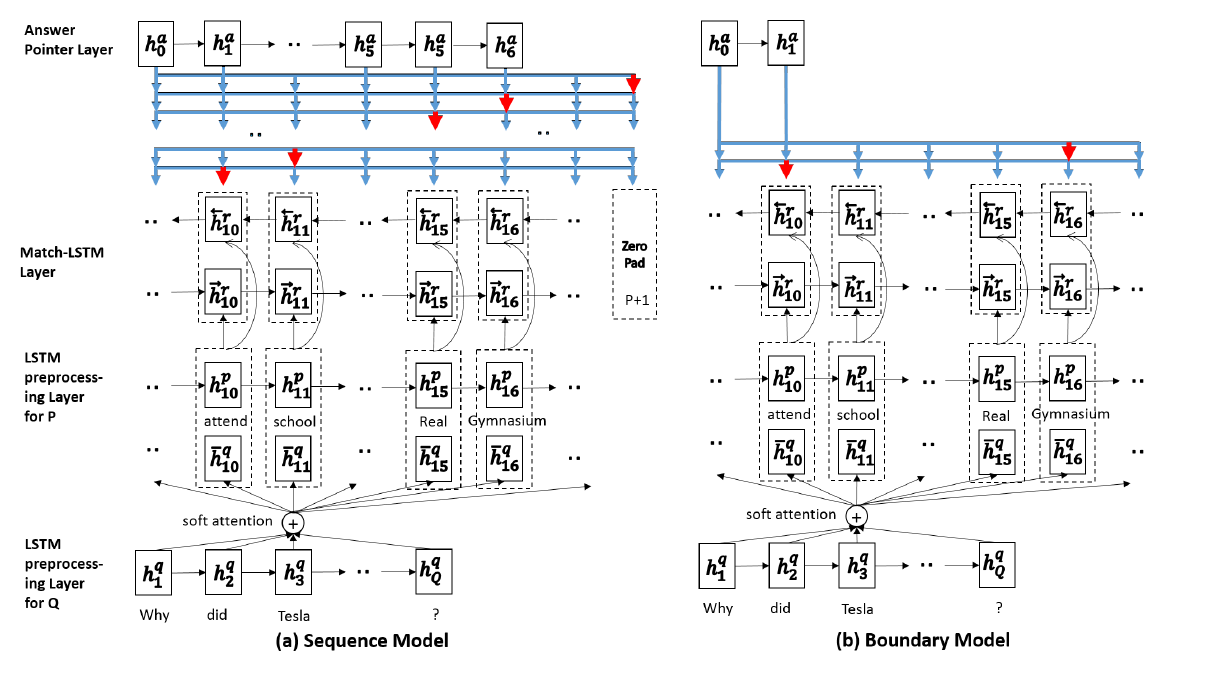
\includegraphics[scale=0.4]{../images/lstmMatch.png}
	         	\caption{Overview of the 2 approaches by \citep{lstmhu2016question}, showing the Sequence Model on the left and the Boundary Model on the right.}\label{lstmMatch}
	         \end{figure}

		It is important to highlight that the sequence model represents the answers as integers in a sequence that refer to the position of the selected token in the original passage. The Ans-Ptr layer models these sequentially as well. For the purposes of this thesis we will focus on the boundary model from the paper by \citep{lstmhu2016question}. As we can see from table \ref{tableMatchLSTM}, the results are significantly better for SQuAD 1.1 dataset. Further enhancements to this have been made and various other models have come out on top, however this paper pioneered the use of a bidirectional Ans-Ptr approach.
		\begin{table}[!htbp]
			\centering
		\resizebox{\columnwidth}{!}{
			\begin{tabular}{lcccccc}
			\hline & $l$ & $|\theta|$ & \multicolumn{2}{c}{ Exact Match } & \multicolumn{2}{c}{ F1 }\\
			& & & Dev & Test & Dev & Test \\
			\hline Random Guess & $-$ & 0 & $1.1$ & $1.3$ & $4.1$ & $4.3$ \\
			Logistic Regression & $-$ & $-$ & $40.0$ & $40.4$ & $51.0$ & $51.0$ \\
			DCR & $-$ & $-$ & $62.5$ & $62.5$ & $71.2$ & $71.0$ \\
			\hline Match-LSTM with Ans-Ptr (Sequence) & 150 & $882 \mathrm{~K}$ & $54.4$ & $-$ & $68.2$ & $-$ \\
			Match-LSTM with Ans-Ptr (Boundary) & 150 & $882 \mathrm{~K}$ & $61.1$ & $-$ & $71.2$ & $-$ \\
			Match-LSTM with Ans-Ptr (Boundary+Search) & 150 & $882 \mathrm{~K}$ & $63.0$ & $-$ & $72.7$ & $-$ \\
			Match-LSTM with Ans-Ptr (Boundary+Search) & 300 & $3.2 \mathrm{M}$ & $63.1$ & $-$ & $72.7$ & $-$ \\
			Match-LSTM with Ans-Ptr (Boundary+Search+b) & 150 & $1.1 \mathrm{M}$ & $63.4$ & $-$ & $73.0$ & $-$ \\
			Match-LSTM with Bi-Ans-Ptr (Boundary+Search+b) & 150 & $1.4 \mathrm{M}$ & $\mathbf{6 4 . 1}$ & $\mathbf{6 4 . 7}$ & $\mathbf{7 3 . 9}$ & $\mathbf{7 3 . 7}$ \\
			\hline Match-LSTM with Ans-Ptr (Boundary+Search+en) & 150 & $882 \mathrm{~K}$ & $\mathbf{6 7 . 6}$ & $\mathbf{6 7 . 9}$ & $\mathbf{7 6 . 8}$ & $\mathbf{7 7 . 0}$ \\
			\hline
		\end{tabular}
	}
		\caption{Experiment results from \citep{lstmhu2016question} that highlight various configurations implemented. The best being Match-LSTM with Ans-Ptr using a boundary, search and ensemble technique.}\label{tableMatchLSTM}
		\end{table}
		\begin{figure}[!h]
			\centering
			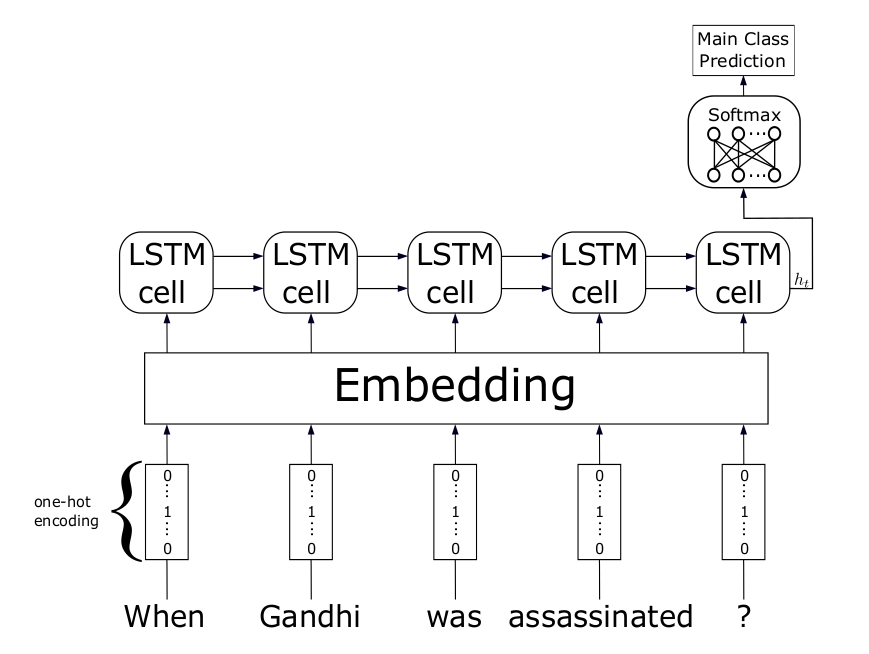
\includegraphics[scale=0.35]{../images/lstm-intent1.png}
			\caption{Basic classification model using LSTM \citep{lstmintent}}\label{lstmIntent1}
		\end{figure}
	     Our research has shown that this approach hasn't yet been applied to the SQuAD 2.0 dataset. In chapter \ref{c3researchmeth}, section \ref{c33} we will hypothesize the implementation of this approach along with the use of Transformers, which are covered in the next section.

         The final piece of research to look at in this section is by \citep{lstmintent} titled \textit{Intent Classification in Question-Answering Using LSTM Architectures}. The approach followed is similar to \citep{lstmSubilstm}, using GloVe embeddings, allowing for prefixes to be added and generating word closeness and using a supervised learning technique. In fig. \ref{lstmIntent1} it can be observed how applying one-hot encoding, followed by GloVe embedding before reaching the LSTM layer and using a Softmax activation layer at one prediction classes allows the model to generate better predictions on the TREC \citep{trec} dataset.

		In fig. \ref{lstmIntent2} we see the implementation of a padding layer at the end of each question and adding a subclass prediction strategy at the end of each prediction. This is done to gain better contextual understanding of the question. The subclass acts as a specialization class while the main class acts as a generalization class, therefore narrowing the context while maintaining global outlook.
		\begin{figure}[!h]
			\centering
			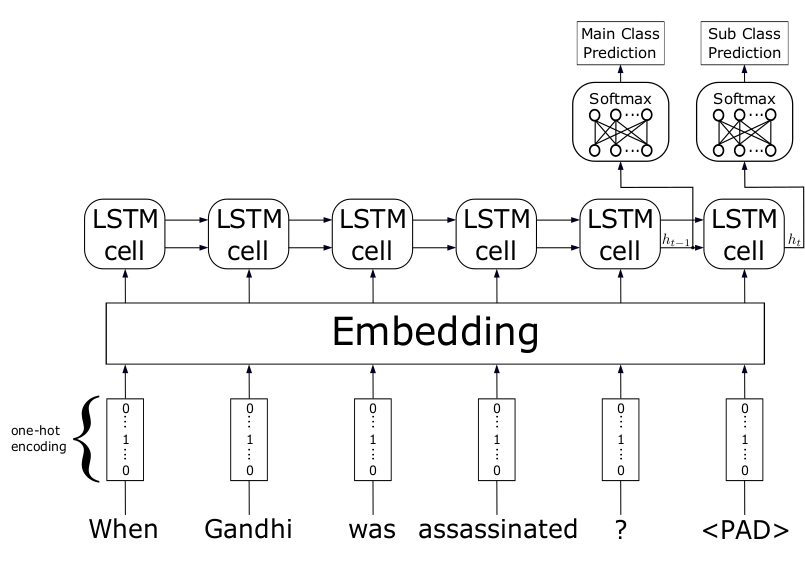
\includegraphics[scale=0.35]{../images/lstm-intent2.png}
			\caption{Basic classification model using RNNs \citep{lstmintent}}\label{lstmIntent2}
		\end{figure}
		To verify their results \citep{lstmintent} implemented a prototype responder by adding a biLSTM on top of the LSTM layer seen in figs. \ref{lstmIntent1} and \ref{lstmIntent2}.  The biLSTM model uses the predictions from the previous layer, both main and subclass predictions, and combines them to form the final output.

		\subsection{Critical Issues in LSTMs}\label{c2criticalissues}

		From the literature reviewed so far, it has become apparent that LSTMs generate a view of the world in a very sequential manner. While successful in managing banishing gradients and generating better, contextually relevant results, LSTMs or even biLSTMs aren't entirely correct, with none of the models achieving over 90\% accuracy across various datasets consistently. LSTMs suffer from another fatal flaw, their sequential nature makes it extremely difficult to parallelize the work and this leads to extended training times, out of memory errors etc.

	    \section{Transformers}\label{23}

	    	The previous section highlighted some key advancements in the field of machine comprehension and LSTMs, however, not a lot changed for almost two decades in the field of NLP based machine comprehension tasks architecturally. Since their introduction in 1997, LSTMs \citep{lstmoriginal} have been the base architecture for countless applications. However, as we noted in section \ref{c2criticalissues}, LSTMs have some critical drawbacks.

			\textit{Transformers} were introduced in late 2017 by \citep{atayl} and have become a very reliable way to implement various NLP based tasks. The basic architecture for which can be seen in fig. \ref{transformerArchitecture}.
			\begin{figure}[h!]
				\centering
				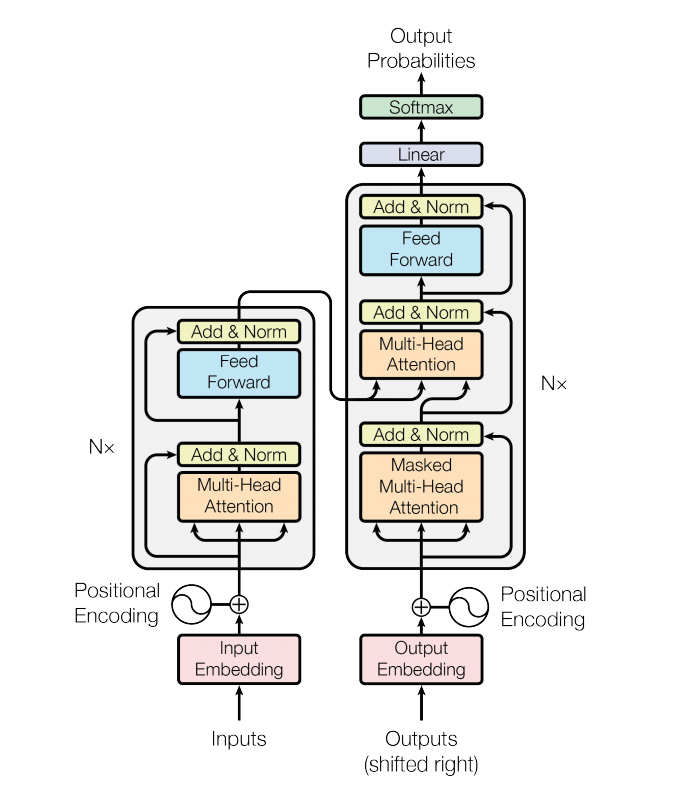
\includegraphics[scale=0.4]{../images/transformer.png}
				\caption{Transformer Architecture built by \citep{atayl}}\label{transformerArchitecture}
			\end{figure}
	        Recurrent models usually adopt a combination approach where they take symbol position of the input and output positions along with the computation. This helps them align positions to steps in computation time and generate a sequence of hidden states $ h_{t} $, which is a function of the previous hidden state $ h_{t-1}$ and the input function $ t $.  This inherently sequential nature of RNNs causes memory issues, leading to reduced batch sizes.

			The architecture for a \textit{Transformer} in this paper is outlined as having an encoder that maps input sequences to a continuous representation. The architecture can be seen in Fig. \ref{transformerArchitecture}. This is then decoded into an output sequence of symbols one at a time. Each step is auto-regressive, ie. it consumes the previously generated symbols as additional input when creating the next. This is similar to an ensemble model. Stacks of 6 encoder and 6 decoder layers is used.\\
			Each encoder layer has 2 sub-layers of a multi-head self-attention and the other a simple, position-wise fully connected feed-forward network layer. The output from each encoder layer can be represented as $  LayerNorm(x + Sublayer(x)) $, where $ Sublayer(x) $ is the function implemented by the sub-layers in the model. Additionally, supporting residual connections is handled by producing outputs of dimension $ d_{model}=512 $.

			The decoder layer is similar to the encoder layer and has an additional 3rd sub-layer that performs multi-head attention over the output of the encoders. To ensure that the output layer isn't affected by the output of residual connections from the sub-layers, a normalization layer is implemented at the end. Masking the subsequent positions and offsetting the output by 1 position ensures that the predictions for position $ i $ can only depend on outputs from previous positions.

            The \textit{Transformer} architecture was the first one to implement a self-attention based transduction model to compute input and output representations without the use of convolution or sequence-aligned networks.

			One of the key features in a Transformer architectures is \textit{self-attention}, which is covered in-depth in section \ref{231}.

			\subsection{Self Attention}\label{231}

            In their paper ``Attention Is All You Need", \citep{atayl} highlight that \textit{self-attention} is a key piece of the puzzle. This is due to several reasons such as the ability to parallelize computation, reduce total complexity per layer and the reduced path lengths between various long-range dependencies in the network. It is easier to learn about these dependencies if the distance between them is shorter.
            Thus, the transformer also computes the length of the longest path between any two input-output positions.

            The attention mechanism was designed by \citep{attentioneMech} to solve a critical issue with encoder-decoder architecture dependent LSTM and RNN based models. As has been highlighted before, LSTMs suffer from an inability to retain long-range sequence dependencies. Using a (soft)-search approach allows the model to look for parts that are relevant to predicting an output sequence, rather than forming all the segments of a sentence produces better results than existing fixed-length encoder-decoder models.
            The (soft)-search is performed after a prediction is made. This prediction is based on a set of positions for the source sentence, where the target word has the highest concentration of context vectors associated with previously generated target words. Another distinguishing feature of the attention mechanism is that it does not try to encode an entire input sentence to a fixed-length vector. Rather, it encodes the input sentence into sequence vectors that can be adaptively decoded during translation. Thus freeing the model from having to squash a lot of information from the source sentence into a vector of fixed-length.

			The work done in \citep{atayl} modified that attention mechanism by mapping a query to a set of key-value pairs and developing \textit{self-attention}. To understand self attention take an example sentence like:
            \\\\
            \textit{``The lion was resting in the shade because it was tired after hunting."}\\

             While this is a perfectly normal sentence to a human being, a computer does not know what ``it" means and that ``it" refers to the ``lion" in the second half of this sentence. Self- attention allows a Transformer to understand that the word ``it" refers to the ``lion" in this context.
             In fig. \ref{multiHeadAttention} shows how \citep{atayl} modified the attention mechanism.
			\begin{figure}[h!]
				\centering
				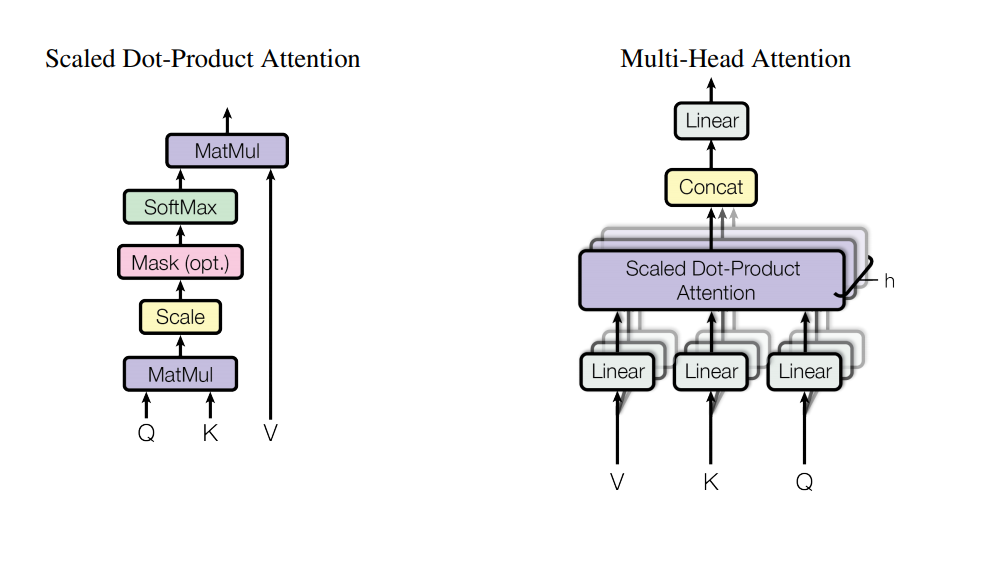
\includegraphics[scale=0.4]{../images/multihead.png}
				\caption{Scale Dot and Multi-Head Attention Models \citep{atayl}}\label{multiHeadAttention}
			\end{figure}

            The ``Scaled Dot-Product Attention" layer implemented in the transformer works by computing the dot products of all the input query with all the keys, divide it by the dimension of the keys and finally apply a softmax function to obtain the weights. This can be represented as:

            \begin{equation}\label{attentionEq}
                Attention(Q,K,V)=softmax\bigg(\dfrac{QK^{T}}{\sqrt{d_k}}\bigg)V
            \end{equation}
            where $ K, V $ are the matrices containing the keys and values respectively, and $ Q $ is the set of queries. The dimension of the keys is given by $ d_k $. The dot product is used because it is more efficient than the additive attention product and is faster as well \citep{atayl}.

            Instead of using single attention, the transformer implements \textit{multi-head} attention.  Multi-head attention, which can be seen in fig. \ref{multiHeadAttention} on the right, allows for the model to simultaneously gather information from various different representations in different subspaces and positions.
            \begin{equation}\label{multiheadEQ}
            \begin{aligned}
               \text{MultiHead}(Q,K,V) = Concat(head_1,...,head_h)W^O \\
                \text{where head}_{\mathrm{i}}=\text { Attention }\left(Q W_{i}^{Q}, K W_{i}^{K}, V W_{i}^{V}\right)
            \end{aligned}
           \end{equation}

            Matrices $W_{i}^{Q} \in \mathbb{R}^{d_{\text {model }} \times d_{k}}, W_{i}^{K} \in \mathbb{R}^{d_{\text {model }} \times d_{k}}, W_{i}^{V} \in \mathbb{R}^{d_{\text {mod } 1} \times d_{v}}$ and $W^{O} \in \mathbb{R}^{h d_{v} \times d_{\text {model }}}$ represent the projection parameters. They also implemented $h=8$ parallel attention/head layers. The reduced dimensionality of each head with $d_{k}=d_{v}=d_{\text {model }} / h=64$ means that the total cost is similar to a fully connected, single-head attention layer.
            The evaluations performed on the Wall Street Journal dataset\citep{wsj}, using 40k sentences, showed that even without task-specific tuning the model had better results with a fraction of the training cost.

            The advantages of the Transformer architecture are clearly evident over the standard RNN based LSTMs and other architectures. Experiments on the WMT 2014 English to German translation \citep{wmt} using the big transformer showed a significant jump in BLEU score 28.4 over various other seq2seq models and even combined ensemble models which earlier had a highest score of 26.36 using a ConvS2S Ensemble \citep{convs2s}.


		\subsection{Improvements of Transformer Architectures}\label{232}

            Transformers have significant advantages as highlighted earlier. Improvements to the basic architecture are discussed below.
		\subsubsection{BERT}\label{2321}

			The paper on \textit{Bidirectional Encoder Representations from Transformers} (BERT) \citep{bert}, introduces a new language model. This model is truly fascinating in many ways. First and foremost it is designed to pre-train deep bidirectional representations using unlabelled data. This is done by jointly conditioning context in all layers to the right and left. This pre-training allows the model to be fine-tuned simply using one additional output layer. These features make this model conceptually simple and very powerful empirically.

			BERT employs language pre-training \citep{dai, deepContextualized, radford2018improving} which has shown significant advantages in many applications e.g. paraphrasing, language level inference etc. These tasks aim to highlight the relationships between sentences through contextual understanding as well as by using tokenized outputs. BERT improves on the fine-tuning tasks that are important to performing
			\begin{figure}[h!]
				\centering
				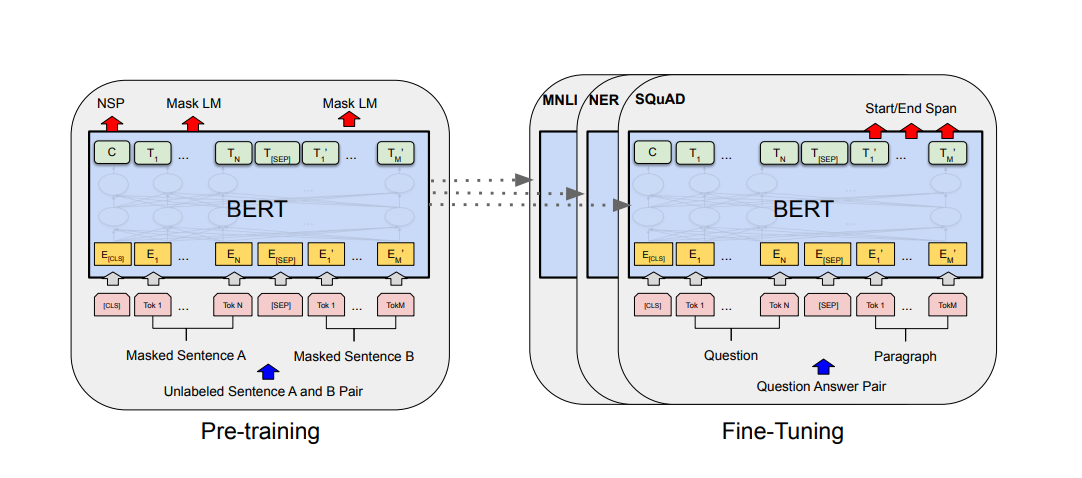
\includegraphics[scale=0.35]{../images/BERT.png}
				\caption{Pre-training and Fine Tuning procedures for BERT \citep{bert}}\label{bertPretraining}
			\end{figure}

			BERT was tested on The General Language Understanding Evaluation (GLUE) benchmark \citep{wang} which has a large number of diverse NLU tasks.
			BERT performed extremely well on the 11 NLP tasks that it ran against. It showed an average accuracy improvement of 4.5\% and 7\% when compared to the previous state of the art models. Results of BERT and its significant gains make it one of the best candidate models for NLU tasks.

%	       \subsubsection{ALBERT}\label{albertLitrev}
%	    \citep{albert}

%	     \subsubsection{ROBERTA}\label{robertaLitrev}
%	      \citep{roberta}

	    \subsubsection{DistilBERT}\label{distilLitrev}
	    The DistilBERT model by \citep{distil} was created with a few factors in  mind such as model size, complexity, ability to generalize tasks and the high environmental cost of running larger models. Models like RoBerta \citep{roberta}, BERT \citep{bert} etc. have several hundred million model parameters that take particularly longer to train, even through use of advanced pre-training techniques.

	    Larger models often tend to exponential increase model computational requirements \citep{schwarts}, these models also fail to generalize. The DistilBERT model shows that by applying a triple loss function on top of a smaller Transformer \citep{atayl} that is trained using a knowledge distillation compression technique \citep{knowledgeDistilation} can provide similar results in 60\% less time.

	    The work proposes a \textit{``Student-Teacher"} architecture. The DistilBERT model, which is the student architecture, has the same kind of layout as the BERT model but without the tokenized embeddings and the pooler architecture, with a further reduction in the number of layers.

	    Experiments showed that training a DistilBERT model produced similar results to BERT-base model but in a lot less time than its parent architecture BERT. The model is 0.6\% behind BERT on the IMDB and only 3.9\% behind BERT on the SQuAD 1 dataset.

	    These speed and accuracy advantages make this model and architecure worthy of being explored further and will serve as the basis of the improvements suggested in this thesis.



    \chapter{Research Methodology}\label{c3researchmeth}


    \section{Data Selection}\label{c31}

    	The Stanford Question Answering Dataset (SQuAD) 2.0 has been chosen as the dataset for the experiments proposed. This is as a reading comprehension dataset based on Wikipedia articles. It is based on questions posed by crowd-workers on a set of articles. The answer to every question is a segment of text or span, from the corresponding reading passage, or the question might be unanswerable \citep{dataset}.

    	The dataset consists of over 150,000 questions. Split into 100,000 answerable and 50,000+ unanswerable question, which were written to look similar to unanswerable questions. The challenge being that a model should be able to correctly answer the answerable questions and abstain from answering the unanswerable ones.
	    The dataset is freely available as a part of the Transformers package in python or it can be downloaded from the SQuAD 2.0 website \citep{squad}.

	    To effectively use this dataset for our purposes, let us first take a look at what its contents look like below.\\ \\
	    \noindent\fbox{
	    	\parbox{\textwidth}{\textbf{Context:}\textit{``The Normans (Norman: Nourmands; French: Normands; Latin: Normanni) were the people who in the 10th and 11th centuries gave their name to Normandy, a region in France. They were descended from Norse (``Norman" comes from ``Norseman") raiders and pirates from Denmark, Iceland and Norway who, under their leader Rollo, agreed to swear fealty to King Charles III of West Francia."}\\
	    		\textbf{Question: } \textit{Who was the Norse leader?}\\
	    		\textbf{Answer: } \textit{Rollo}}
	    }
	    \newline
	    \newline

	    The answer to the aforementioned question is quite simple for humans to comprehend. The challenge is for computational systems is to contextualize this and make it machine-understandable so that the produced model can answer it correctly.
	    The dataset consists of various kinds of English language examples like negation, antonyms, entity swaps, impossible conditions to answer, answerable, etc. making the dataset a well-balanced one.
	    It is important to prepare this dataset appropriately, this will be done

	    \begin{enumerate}
	    	\item Data splitting into separate Question, Answer and Context lists for use for both the training data and the validation data
	    	\item Tokenization of the split data to generate ``context-question" pairs
	    	\item Generating indexes for when an answer begins and ends in the dataset
	    	\item Adding answer and context tokens based on their encoded positions
	    \end{enumerate}

        The SQuAD 2.0 Dataset \citep{dataset}, was developed with funding from Facebook to help address some major issues with existing datasets. Most datasets focus on questions that can be easily answered or use of    automatically generated, unanswerable questions which are easily identifiable.\\
        The SQuAD 2.0 dataset resolves this by combining the SQuAD dataset along with 50,000 crowd worker generated unanswerable questions. The key feature of these being that the unanswerable questions must look similar to answerable ones. For a model to be successful on this new dataset, it must be able to answer all possibly answerable questions as well as determine when no answers are provided for a question in the given paragraph and abstain from answering. A comparative study was done for a Natural Language Understanding(NLU) task that obtained an 86\% score on SQuAD 1.1, only got 66\% on the new 2.0 dataset.
        The dataset helps bridge the gap between true NLU and machine understanding by using the concept of Relevance. Through comparisons with various datasets such as RACE, MCTest, QASENT etc. they have identified the missing links like negative examples, antonyms and helped fill the gap. This dataset forces the models to understand whether a paragraph span has the answer to the question posed.

		\begin{table}[h!]
		              \centering
		                \begin{tabular}{|l|l|l|}
		                    \hline
		                     & SQuAD 1.1 &  SQuAD 2.0 \\
		                    \hline
		                    \textbf{Train} & & \\
		                        Total Examples & 87,599 &  130,319 \\
		                        Negative Examples & 0 & 43,498 \\
		                        Total articles & 442 & 442 \\
		                        Articles with negatives & 0 & 285 \\
		                    \hline
		                    \textbf{Development} & & \\
		                        Total Examples & 10,570 &  11,873 \\
		                        Negative Examples & 0 & 5,945 \\
		                        Total articles & 48 & 35 \\
		                        Articles with negatives & 0 & 35 \\
		                    \hline
		                    \textbf{Test} &  & \\
		                        Total Examples & 9,533 & 8,862 \\
		                        Negative Examples & 0 & 4,332 \\
		                        Total articles & 46 & 28 \\
		                        Articles with negatives & 0 & 28 \\
		                    \hline
		                \end{tabular}
		                \caption{Comparison of  SQuAD 2.0 to SQuAD 1.1\citep{dataset}.}\label{datasetDescription}
		 \end{table}

    Table \ref{datasetDescription} shows the difference between SQuAD 1.1 and SQuAD 2.0 datasets.

    \section{Research Hypothesis}\label{c33}
    The hypothesis of this research is that implementing a self attention based Transformer model with:
    \begin{itemize}
    	\item Glove embeddings
    	\item BERT base \citep{bert} type Transformer model
    	\item Answer pointer output layer\citep{lstmPointer, lstmhu2016question}
    \end{itemize}

	Will help improve the prediction capability of the transformer architecture.

	The DistilBERT model \citep{distil}, which is a lighter, distilled version of the BERT model, and has 40\% less parameters at 66 million, instead of 110 million in BERT, as discussed in \citep{bert}, will be customized with the implementation of the answer pointer layer to generate answers for the questions posed.


	\section{Model Evaluation Metrics}\label{33}

		To successfully evaluate the model two metrics will be used. The \textit{F1 - Score} and \textit{Exact Match Score} will be used to measure the success of the model developed. While accuracy is a good score to measure how well a model is performing, the problem with accuracy is that it is prone to overfitting, and underfitting, which might lead to great accuracy scores but real world predictions wont be as accurate.

		Accuracy also doesn't work because it is a simplistic probability metric that assumes both false positives and false negatives have an equal weight in predicting the outcome as shown in eq. \ref{accuracy}.
				\begin{equation}\label{accuracy}
			Accuracy = \small \dfrac{True Positive + True Negative}{True Positive + False Positive + True Negative + False Negative}
		\end{equation}

		Outlined below are some reasons why accuracy is not a good measure:
		\begin{enumerate}
			\item \textbf{Class Imbalance}
			\item \textbf{Prone to Over and Under-fitting}
		\end{enumerate}

	\textbf{Precision} is the probability of identifying a correct positive outcome from all the predicted positive outcomes. Precision is used for cases when the cost of a false positive has a very high negative impact.
	\begin{equation}\label{precision}
		Precision = \dfrac{True Positive}{True Positive +  False Positive }
	\end{equation}

	\textbf{Recall} is defined as the probability of a correctly identifying a positive outcome from all the positive outcomes. Recall is very important in cases where the cost of negative responses or false negatives is high.
		\begin{equation}\label{recall}
		Recall = \dfrac{True Positive}{True Positive +  False Negative }
	\end{equation}

	\textbf{F1 Score } is the harmonic mean of recall and precision. It is used as an evaluation metric in places where the impact of both false positives and negatives is very high.
		\begin{equation}\label{f1}
		F1 = 2 \times \dfrac{Precision \times Recall}{Precision + Recall}
	\end{equation}

	\textbf{Exact Match} is a binary metric, i.e. it is 1 if the predicted answer matches the expected answer and 0 if it doesn't.

	\section{Research Flow Diagram}\label{c34}
	 To be able to achieve the objectives set out in the previous chapters, it is important to organize the research in such a way that it achieves its objective. This is represented in the research flow diagram \ref{researchFlow}.

	\begin{figure*}
		\begin{center}
			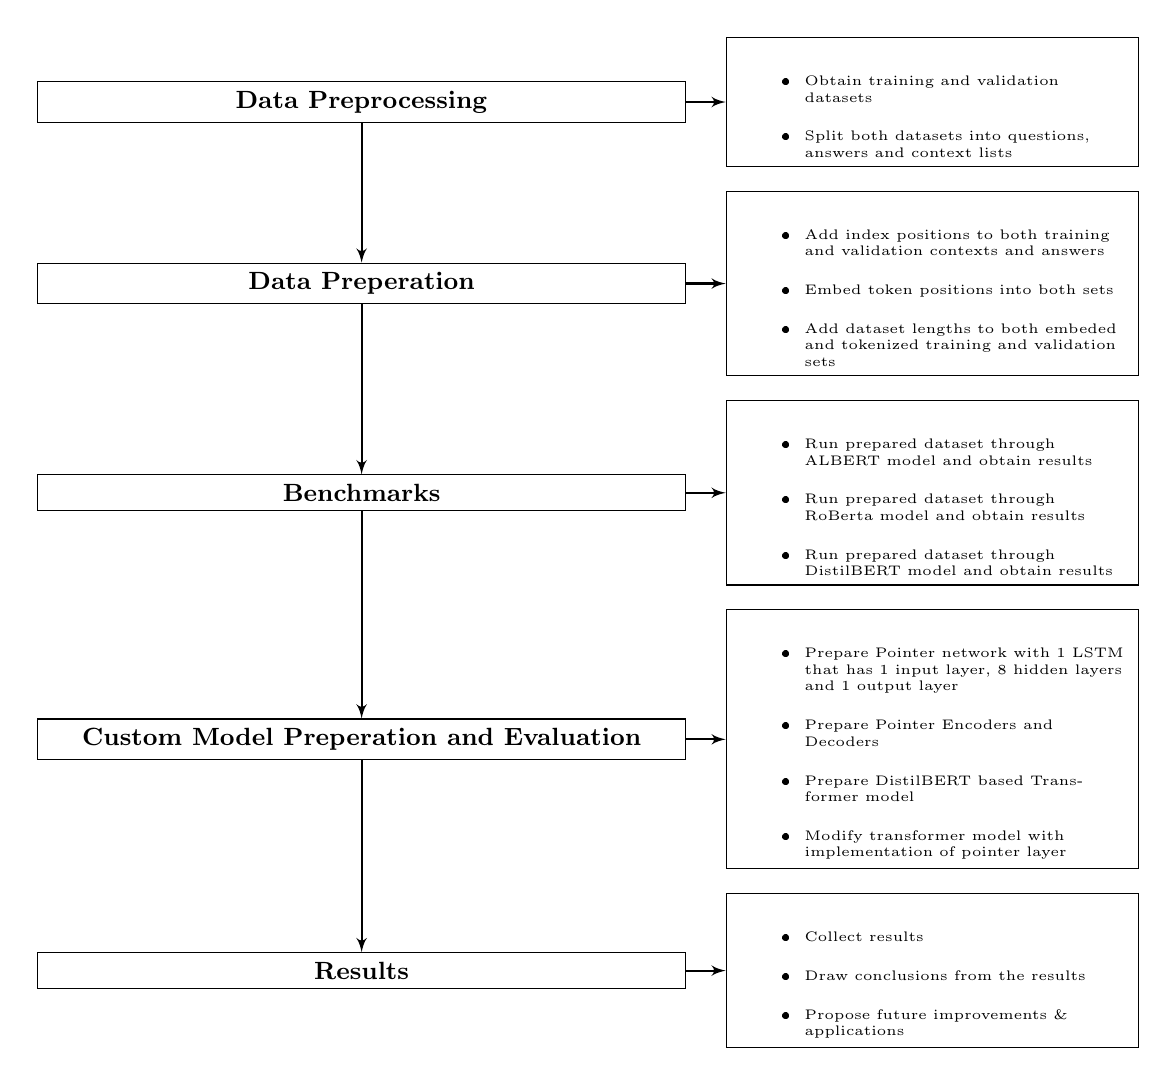
\begin{tikzpicture}[auto,
				%decision/.style={diamond, draw=black, thick, fill=white,
				%text width=8em, text badly centered,
				%inner sep=1pt, font=\sffamily\small},
				block_center/.style ={rectangle, draw=black,
					text width=8cm, text badly centered,font=\small,},
				block_left/.style ={rectangle, draw=black,
					text width=5cm, text centered,font=\tiny},
				line/.style ={draw, thick, -latex', shorten >=0pt}]
				% outlining the flowchart using the PGF/TikZ matrix funtion
				\matrix [column sep=5mm,row sep=3mm] {
					% enrollment - row 1
					\node [block_center] (introduction) {\textbf{Data Preprocessing}};
					& \node [block_left] (introductionLeft) {\begin{itemize}
							\item Obtain training and validation datasets
							\item Split both datasets into questions, answers and context lists
					\end{itemize}}; \\
					% enrollment - row 2
					\node [block_center] (litreview) {\textbf{Data Preperation}};
					& \node [block_left] (litreviewleft) {\begin{itemize}
							\item Add index positions to both training and validation contexts and answers
							\item Embed token positions into both sets
							\item Add dataset lengths to both embeded and tokenized training and validation sets
					\end{itemize}}; \\
					% enrollment - row 3
					\node [block_center] (researchMeth) {\textbf{Benchmarks}};
					& \node [block_left] (researchMethleft) {\begin{itemize}
							\item Run prepared dataset through ALBERT model and obtain results
							\item Run prepared dataset through RoBerta model and obtain results
							\item Run prepared dataset through DistilBERT model and obtain results
					\end{itemize}}; \\
					% enrollment - row 2
					\node [block_center] (dc) {\textbf{Custom Model Preperation and Evaluation}};
					& \node [block_left] (dcleft) {\begin{itemize}
							\item Prepare Pointer network with 1 LSTM that has 1 input layer, 8 hidden layers and 1 output layer
							\item Prepare Pointer Encoders and Decoders
							\item Prepare DistilBERT based Transformer model
							\item Modify transformer model with implementation of pointer layer
					\end{itemize}}; \\
					% enrollment - row 2
					\node [block_center] (results) {\textbf{Results}};
					& \node [block_left] (resultsleft) {\begin{itemize}
							\item Collect results
							\item Draw conclusions from the results
							\item Propose future improvements \& applications
					\end{itemize}}; \\
				};% end matrix
				% connecting nodes with paths
				\begin{scope}[every path/.style=line]
					% paths for enrollemnt rows
					\path (introduction)   -- (introductionLeft);
					\path (introduction)   -- (litreview);
					\path (litreview) -- (litreviewleft);
					\path (litreview) -- (researchMeth);
					\path (researchMeth)  -- (researchMethleft);
					\path (researchMeth) -- (dc);
					\path (dc)  -- (dcleft);
					\path (dc)  -- (results);
					\path (results)   -- (resultsleft);
				\end{scope}
			\end{tikzpicture}
		\end{center}
		\caption{Research Flow Diagram}\label{researchFlow}
	\end{figure*}


  \chapter{Architecture Creation}\label{c4}

  	The literature reviewed in chapter \ref{c2litrev} highlights some exceptional work that has been done in the field of NLP, LSTM and Transformer architectures. This chapter lays the groundwork for the improvements proposed in chapter \ref{c3researchmeth}. Starting off with a review of the drawbacks of the architectures that have been chosen for benchmarks and comparisons, then the improvements are proposed to a BERT based DistilBERT architecture are mentioned in section \ref{c42}.


       \section{Drawbacks Of Current Architectures}\label{c41}

       The transformer based architectures reviewed in section  and the Bi-LSTM \citep{bilstmHerman} have shown great advantages. However, they suffer from certain flaws that are outlined below:


       \section{Proposed Architecture Improvements}\label{c42}

            The proposed architecture is an implementation of the transformer architecture along with a biLSTM based Answer-Pointer network.

            The DistilBERT model that is available through the Hugging Face Library \citep{hfTransformers}, will be modified with the implementation of an Answer-Pointer network. The hypothesis is that by passing the results from Answer-Pointer layer to a DistilBERT based architecture will provide better results since it will already have been encoded with output pointer positions.

            To achieve this the Answer-Pointer based network is designed initially with 1 LSTM cell containing 8 hidden layers and one output layer. This is described in detail section \ref{c421}.

            The process begins by serving tokenized inputs that are created as a part of pre-processing the input data and embedding it by using the ``distilbert-base-uncased" pre-trained embeddings from Hugging Face libarary. Then the input is then fed to the ``DistilBertForQuestionAnsweringC" class, which is the modified class from the Hugging Face Transformers library mentioned before.

            The DistilBertForQuestionAnsweringC class takes a pre-trained model config file as input along with the embedded inputs, passes them through a linear layer and a dropout layer. These processed outputs are then processesed through Encoder and Decoder layers that allow the model to process and produce relevant results.

                             	\begin{figure*}
                             		\begin{center}
                             			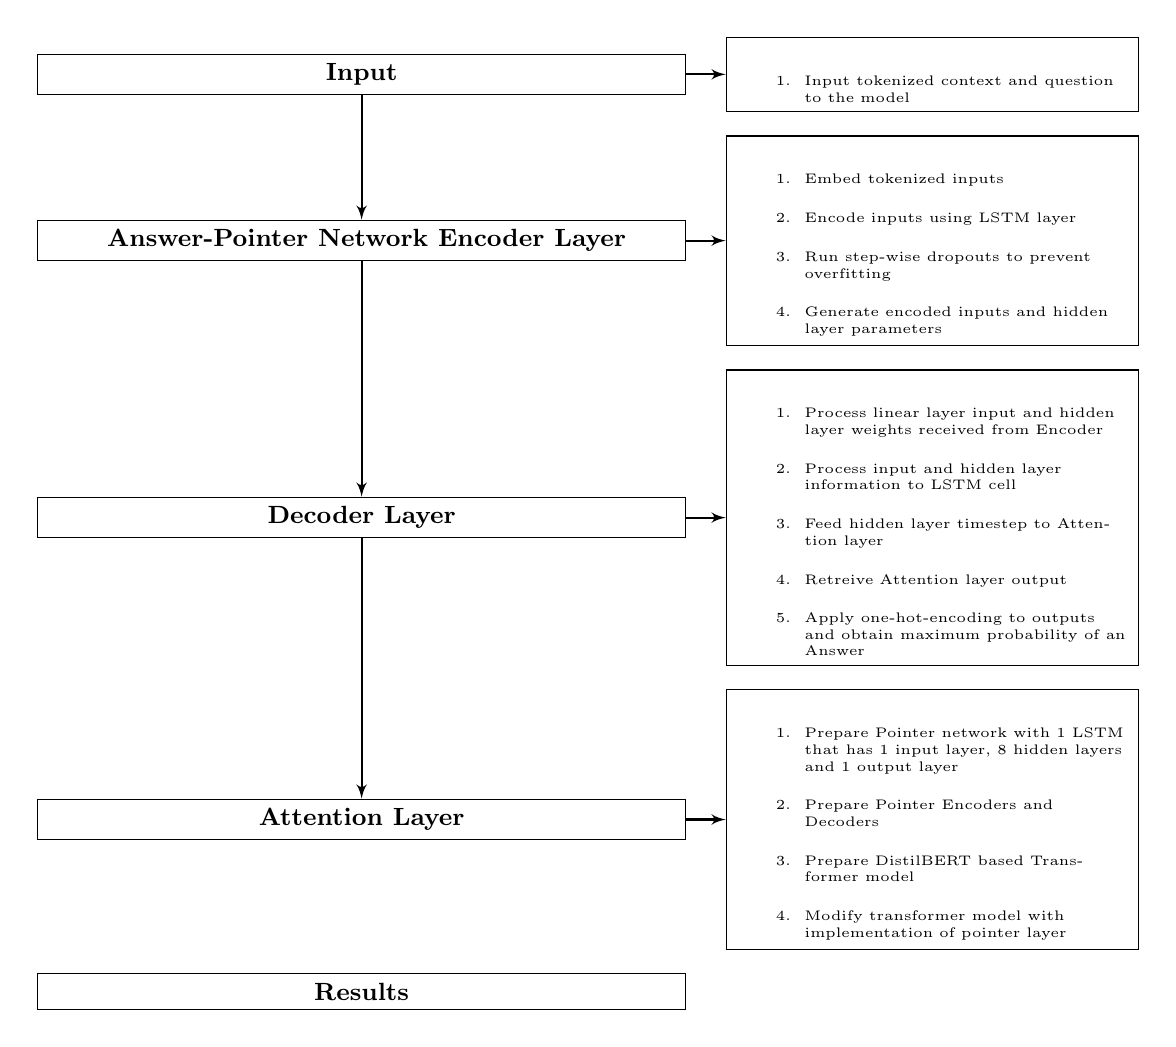
\begin{tikzpicture}[auto,
                             				%decision/.style={diamond, draw=black, thick, fill=white,
                             				%text width=8em, text badly centered,
                             				%inner sep=1pt, font=\sffamily\small},
                             				block_center/.style ={rectangle, draw=black,
                             					text width=8cm, text badly centered,font=\small,},
                             				block_left/.style ={rectangle, draw=black,
                             					text width=5cm, text centered,font=\tiny},
                             				line/.style ={draw, thick, -latex', shorten >=0pt}]
                                             \tikzstyle{arrow} = [thick,->,>=stealth]

                             				% outlining the flowchart using the PGF/TikZ matrix funtion
                             				\matrix [column sep=5mm,row sep=3mm] {
                             					% enrollment - row 1
                             					\node [block_center] (input) {\textbf{Input}};
                             					& \node [block_left] (inputl) {\begin{enumerate}
                             							\item Input tokenized context and question to the model
                             					\end{enumerate}}; \\
                             					% enrollment - row 2
                             					\node [block_center] (el) {\textbf{ Answer-Pointer Network Encoder Layer}};
                             					& \node [block_left] (ell) {\begin{enumerate}
                             							\item Embed tokenized inputs
                             							\item Encode inputs using LSTM layer
                             							\item Run step-wise dropouts to prevent overfitting
                             							\item Generate encoded inputs and hidden layer parameters
                             					\end{enumerate}}; \\
                             					% enrollment - row 3
                             					\node [block_center] (dl) {\textbf{Decoder Layer}};
                             					& \node [block_left] (dll) {\begin{enumerate}
                             							\item Process linear layer input and hidden layer weights received from Encoder
                             							\item Process input and hidden layer information to LSTM cell
                             							\item Feed hidden layer timestep to Attention layer
                             							\item Retreive Attention layer output
                             							\item Apply one-hot-encoding to outputs and obtain maximum probability of an Answer
                             					\end{enumerate}}; \\
                             					% enrollment - row 2
                             					\node [block_center] (al) {\textbf{Attention Layer}};
                             					& child {\node [block_left] (all) {\begin{enumerate}
                             							\item Prepare Pointer network with 1 LSTM that has 1 input layer, 8 hidden layers and 1 output layer
                             							\item Prepare Pointer Encoders and Decoders
                             							\item Prepare DistilBERT based Transformer model
                             							\item Modify transformer model with implementation of pointer layer
                             					\end{enumerate}};} \\
                             					% enrollment - row 2
                             					\node [block_center] (results) {\textbf{Results}};\\
                             				};% end matrix
                             				% connecting nodes with paths
                             				\begin{scope}[every path/.style=line]
                             					% paths for enrollemnt rows
                             					\path (input)   -- (inputl);
                             					\path (input)   -- (el);
                             					\path (el)   -- (ell);
                             					\path (el) -- (dl);
                             					\path (dl) -- (dll);
                             					\path (dl)  -- (al);
                             					\path (al) -- (all);
                             					\path (dl)  (results);
                             				\end{scope}
                             			\end{tikzpicture}
                             		\end{center}
                             		\caption{BOLT Data Flow Diagram}\label{dataflowDiagram}
                             	\end{figure*}

            \subsection{BERT Optimized LSTM Transformer, BOLT}\label{c421}

                The BOLT model begins with the implementation of a Pointer network that feeds the output to the DistilBERT implementation. To better understand the flow of this model a flow diagram is presented in \ref{dataflowDiagram}.

                The Answer-Pointer network consists of 4 main parts, an Encoder layer, an Attention layer, a biLSTM layer and a Decoder layer. The implementation of this is done using PyTorch and inspired by work from \citep{pointernetGit}. This was extremely helpful as Pointer networks aren't readily available from libraries.

                The network begins with taking an input sequence of embeddings and passing it through a linear layer that takes input and output dimensions. The embedded inputs are then passed through the Encoder layer.

                The Encoder layer consists of LSTMs with dropout layers. The LSTM layers are doubled if implemented in biLSTM mode. The dropuout layer helps reset the input dimensions to 0 before taking the next set of inputs, this helps in preventing overfitting. The dropout layer also controls the rate at which the values are set to 0 and is a value between 0-1, with a default of 0.5. Essentially, the dropout layer retains only a small percentage of the outputs from a hidden layer, thus preventing an already large model from gaining more size.

                The LSTM layer processes the input embeddings, encodes them further appropriately and produces encoded outputs for the decoder layer. The Decoder layer is a comprised of several linear layers and an attention layer. The linear layers serve as both input, hidden and output layers, however, the hidden layers are also connected to attention layers that help localize the context of the word in the input question and context.

                The decoder layer generates an output using an internal LSTM layer, thus providing a tuple of output and pointer values plus a separate output of hidden layer weights.These outputs and pointer values are then fed back into the linear output layer of the DistilBERT model.

                The BOLT model uses the existing implementation of the DistilBERT model from the Hugging Face library \citep{hfTransformers} and modifies its base class with an implementation of the Answer Pointer layer mentioned earlier in this chapter.

                The output from that layer is then fed through to the DistilBERT based transformer where it takens the outputs from the Pointer network as input embeddings, applies an attention mask in case the input sequence is smaller in length than the current batch, before finally producing a set of output sequence tokens that serve as pointers to identify which words are the predicted outputs of the model. The architecture of the DistilBERT model is not modified but used as an extension to the pointer network.

    \chapter{Results}\label{c5}

        To establish the improvements hypothesized in the previous section it is important to have a baseline metric. The ALBERT \citep{albert}, RoBERTa \citep{roberta} and DistilBERT \citep{distil} models are available pre-trained through the HuggingFace library \citep{hfTransformers}. The library also provides the SQuAD 2.0 Dataset \citep{dataset} for use. The dataset is also available for download directly and to aid understanding of the data correctly that approach is implemented.

        The code used to prepare the datasets as well as the results gathered are available as examples from the HuggingFace library documentation, some changes have been mde to them to accomodate upgrades from different dependencies.

        For the sake of consistency of the results presented, the experiments were conducted using a Google Colab Pro account with Tesla series GPUs and 16GB of VRAM. Google Colab hosts GPUs in the cloud environment, which impacts performance but is the best alternative to investing and buying a GPU given the silicon shortage and exhorbitant prices in the current market.

        \section{Experiment Data Pre-Processing And Analysis}

        Before performing the experiments on the custom BERT models designed, the SQuAD 2.0 dataset needs to be prepared for use. As outlined chapter \ref{c3researchmeth}, the dataset consists of over 130 thousand questions in the training set.
        Below are some of the steps taken to prepare the dataset and some details from the same:

        \begin{itemize}
        	\item \textbf{Splitting Dataset}: The dataset consists of 2 files ``dev-v2.0.json" and ``train-v2.0.json", which serve as validation and training sets. These consist of questions, relevant contexts and answers, respectively. The dataset is prepared by extracting these into separate data structures(lists) for use.
        	\item \textbf{Training Context}: Upon reading and splitting the data into training contexts, questions and answers, it can be seen that there are 86,821 contexts provided in the training set and 20,302 contexts in the validation set.
        	\item \textbf{Indexing Ends}: The training and validation datasets are then embedded with index position that help identify the answer to the questions in the context layers.
        	\item \textbf{Tokenization}: The training and validation datasets are then embedded with token positions that are obtained from the pre-trained DistilBertTokenizer available from the Hugging Face library.
        	\item \textbf{Training and Validation Datasets}: The encoded datasets are then modified to contain the length of each set as that is required by the modified architecture as well as the base architectures.
        \end{itemize}


     \section{Existing Architecture Benchmarks}\label{c51}

     	Each of the three selected models is put through the same process of data pre-processing, as identified in chapter \ref{c3researchmeth}, this is to ensure consistency across board with all the model types and even the custom model improvements advised.

    	The experiments begin with a review of the ALBERT architecture \citep{albert}, where it is observed that at a batch size of 8 with the AdamW optimizer set to a learning rate of 5e-5, the average epoch time for training takes around 1 hour, 24 minutes at 2.15 iterations/second. Further, the vaidation set takes around 7-12 minutes, depending on the availability of the GPU in the cloud based Google Colab Pro environment.

    	 \begin{figure*}
    		\centering
    		\begin{subfigure}[b]{0.4\textwidth}
    			\centering
    			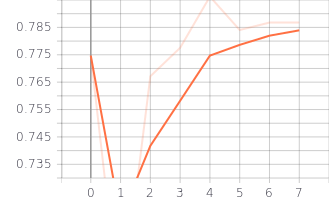
\includegraphics[width=\textwidth]{../images/Albert_Val_F1.png}
    			\caption{\small ALBERT Validation F1 Score}
    			\label{albertf1}
    		\end{subfigure}
    		\hfill
    		\begin{subfigure}[b]{0.4\textwidth}
    			\centering
    			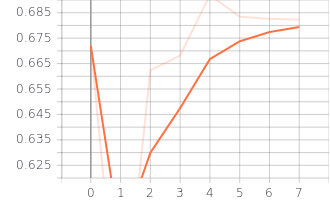
\includegraphics[width=\textwidth]{../images/Albert_Val_EM.png}
    			\caption{\small ALBERT Validation Exact Match}
    			\label{albertem}
    		\end{subfigure}
    		\vskip\baselineskip
    		\begin{subfigure}[b]{0.4\textwidth}
    			\centering
    			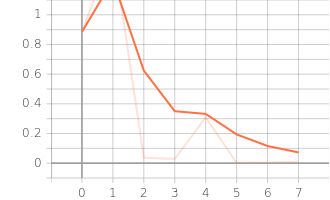
\includegraphics[width=\textwidth]{../images/Albert_Val_Loss.png}
    			\caption{\small ALBERT Validation Loss}
    			\label{albertValLoss}
    		\end{subfigure}
    		\hfill
    		\begin{subfigure}[b]{0.4\textwidth}
    			\centering
    			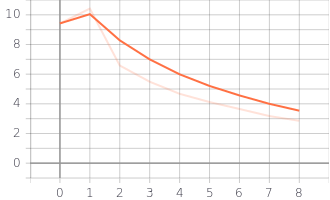
\includegraphics[width=\textwidth]{../images/Albert_Train_Loss.png}
    			\caption{\small ALBERT Training Loss}
    			\label{albertTrainLoss}
    		\end{subfigure}
    		\caption{ALBERT Model Benchmarks}
    		\label{albertBenchmarks}
    	\end{figure*}

    	Figure \ref{albertBenchmarks} shows the various measured parameters across 10 epochs for the ALBERT model. It can be seen from \ref{albertf1} that for the ``albert-base-uncased" pre-trained model class the ALBERT model still suffers from a significant drop in F1 scores in the initial epochs due to the learning rate being set to a very low value of 5e-5. This behaviour is further confirmed by the \ref{albertTrainLoss} and \ref{albertValLoss} graphs where the graph peaks to a higher value for both kinds of losses before tapering down over the remaining epochs.

    	This sudden rise in training and validation loss values that causes poor F1 and exact match scores is purely because of the learning rate. It is seems as though the learning rate is  not appropriate for the batch size of 8, however, for the sake of all the experiments to be baseline it will be observed as such.

    	One interesting observation for the ALBERT benchmarks is that the training loss shown in \ref{albertTrainLoss} shows a consistent, smooth decline while training the model.


    	The final benchmark scores for the ALBERT model at epoch 10 are:
    	\begin{itemize}
    		\item \textbf{F1 Score}: 77.5\%
    		\item \textbf{Exact Match Score}: 67.5\%
    		\item \textbf{Training Loss}:  $\sim$3.7\%
    		\item \textbf{Validation Loss}: $\sim$0.04\%
    	\end{itemize}


\begin{figure*}
	\centering
	\begin{subfigure}[b]{0.4\textwidth}
		\centering
		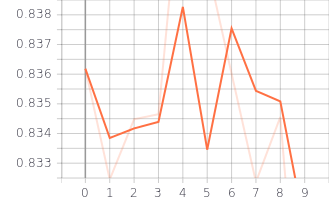
\includegraphics[width=\textwidth]{../images/Roberta_Val_F1.png}
		\caption{\small RoBerta Validation F1 Score}
		\label{robertaf1}
	\end{subfigure}
	\hfill
	\begin{subfigure}[b]{0.4\textwidth}
		\centering
		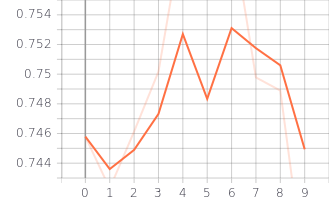
\includegraphics[width=\textwidth]{../images/Roberta_Val_EM.png}
		\caption{\small RoBerta Validation Exact Match}
		\label{robertaem}
	\end{subfigure}
	\vskip\baselineskip
	\begin{subfigure}[b]{0.4\textwidth}
		\centering
		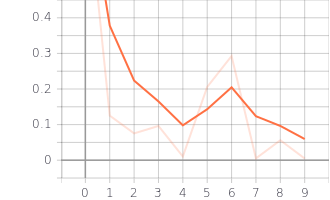
\includegraphics[width=\textwidth]{../images/Roberta_Val_Loss.png}
		\caption{\small RoBerta Validation Loss}
		\label{robertaValLoss}
	\end{subfigure}
	\hfill
	\begin{subfigure}[b]{0.4\textwidth}
		\centering
		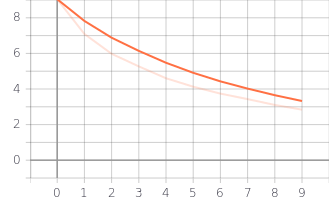
\includegraphics[width=\textwidth]{../images/Roberta_Train_Loss.png}
		\caption{\small RoBerta Training Loss}
		\label{robertaTrainloss}
	\end{subfigure}
	\caption{RoBerta Model Benchmarks}
	\label{robertaBenchmarks}
\end{figure*}

	Figure \ref{robertaBenchmarks} shows the experimental results for the RoBerta architecutre and model. Unlike the ALBERT benchmarks above, the RoBerta benchmark results seem very erratic in nature. The validation F1 and exact match scores for the RoBerta model, while performing significantly better than ALBERT, remain around 83\% and between 74.4 - 75.4\% respectively. This is a roughly 10\% better performance than the ALBERT model, although the training time for the model is around 2 hours per epoch at 1.21 iterations/second. The validation epoch takes around 21 minutes to complete at 4.06 iterations/second.

	This increased training time can be attributed to the almost double number of parameters in the model at 125 million, compared to 66 million in ALBERT when using the ``roberta-base" pre-trained model.

	Similar to the ALBERT model, a consistent and smooth decline in training loss can be observed, as shown in \ref{robertaTrainloss}. The RoBerta model is run using the ``roberta-base" pre-trained class that is similar to the ``albert-base-uncased" class, just optimized by the HuggingFace Team for this model.

	The final benchmark scores for the RoBerta model at epoch 10 are:
	\begin{itemize}
		\item \textbf{F1 Score}:  $\sim$83.3\%
		\item \textbf{Exact Match Score}: 74.6\%
		\item \textbf{Training Loss}:  $\sim$3.7\%
		\item \textbf{Validation Loss}: $\sim$0.5\%
	\end{itemize}


	In figure \ref{distilbertBenchmarks}, the behaviour of the model can be observed to be very different from the other models. The behaviour can be described simply as a combination of the behaviours seen for ALBERT and RoBerta models. Just like in \ref{robertaTrainloss}, the training loss for the DistilBERT model as seen in \ref{distilbertTrainloss} is extremely consistent and smooth in nature, showing a steady decline till the final epoch. training loss and validation loss, fig. \ref{distilbertValLoss} are lower compared to both models above, the validation F1 and exact match scores are not exactly comparable.

	Using the same training criteria of a batch size of 8 and an AdamW optimizer set to a learning rate of 5e-5, it can be seen that the DistilBERT model with performs slightly poorly when compared to ALBERT and RoBerta. However, the time taken to train a DistilBERT model is significanty less than that of RoBerta and ALBERT. One epoch for a DistilBERT model takes approximately 37 minutes to complete, almost half that of ALBERT and 3x less than RoBerta. The validation set takes around 5 minutes as well.

  \begin{figure*}
	\centering
	\begin{subfigure}[b]{0.4\textwidth}
		\centering
		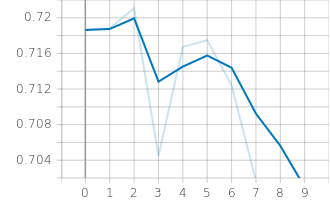
\includegraphics[width=\textwidth]{../images/Distilbert_Val_F1.png}
		\caption{\small DistilBERT Validation F1 Score}
		\label{distilbertf1}
	\end{subfigure}
	\hfill
	\begin{subfigure}[b]{0.4\textwidth}
		\centering
		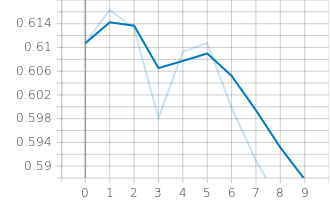
\includegraphics[width=\textwidth]{../images/Distilbert_Val_EM.png}
		\caption{\small DistilBERT Validation Exact Match}
		\label{distilbertaem}
	\end{subfigure}
	\vskip\baselineskip
	\begin{subfigure}[b]{0.4\textwidth}
		\centering
		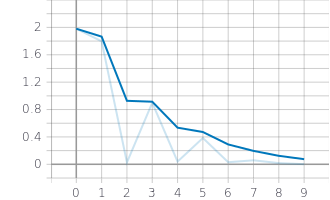
\includegraphics[width=\textwidth]{../images/Distilbert_Val_Loss.png}
		\caption{\small DistilBERT Validation Loss}
		\label{distilbertValLoss}
	\end{subfigure}
	\hfill
	\begin{subfigure}[b]{0.4\textwidth}
		\centering
		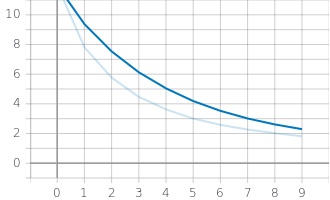
\includegraphics[width=\textwidth]{../images/Distilbert_Train_Loss.png}
		\caption{\small DistilBERT Training Loss}
		\label{distilbertTrainloss}
	\end{subfigure}
	\caption{DistilBERT Model Benchmarks}
	\label{distilbertBenchmarks}
\end{figure*}

	The final benchmark scores for the DistilBERT model at epoch 10 are:
\begin{itemize}
	\item \textbf{F1 Score}:  $\sim$70.4\%
	\item \textbf{Exact Match Score}: $\sim$58.5\%
	\item \textbf{Training Loss}:  $\sim$2.1\%
	\item \textbf{Validation Loss}: $\sim$0.1\%
\end{itemize}

While the results for the DistilBERT model aren't exactly perfect, it does allow for quick prototyping and achieves almost near accurate results.


\section{BOLT Results}\label{c52}

	As discussed in chapter \ref{c4}, the modifications have been applied to the DistilBERT model, specifically the DistilBertModel class offered by the HuggingFace Transformers library \citep{hfTransformers} and a modified implemetation of an Answer Pointer Network designed using PyTorch by \citep{pointernetGit} is used to generate the answer pointer layer results for these custom models. All the custom models utilised the same pre-trained ``DistilBERT-base-uncased" class from the Hugging Face Transformers library.

	\begin{figure}[!h]
		\centering
		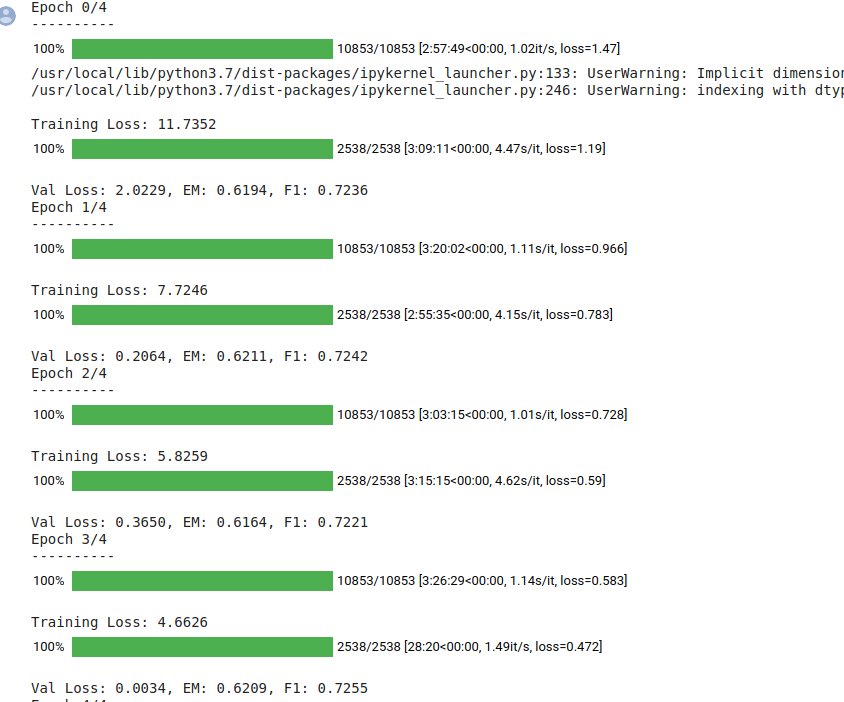
\includegraphics[scale=0.35]{../images/AdamW5e.png}
		\caption{BOLT with AdamW Optimizer at 5e-5 rate}\label{adam5e}
	\end{figure}

	The first figure \ref{adam5e} shows the various epochs for the modified DistilBERT model with the Answer Pointer network implemented with a batch size of 8 and the AdamW optimizer with a learning rate of 5e-5, which  are the same parameters as the benchmark models.

	In figure \ref{adam5e} it can be observed that the model takes significantly longer to train than a regular DistilBERT model which takes around 37 minutes. Though the training and validation times are higher than existing models, the training loss values track consistently down and are comparable to the ones seen in \ref{distilbertTrainloss}. The increased training and validation set times can however be less than the ones shown as there is a significant decrease in the validation set running time towards the 5th epoch. This is quite peculiar and goes to highlight the distributed nature of the cloud based training environment that is Google Colab.

	The F1 scores for the model continuously hover around the 72\% mark, which is a slight improvement over the 70\% mark observed for the benchmarked DistilBERT model as seen in \ref{distilbertf1}.
	The validation loss for the custom model hovers lower than the values in the DistilBERT model as well.

	In the next experiment, shown in fig. \ref{adam3e}, a different learning rate is used with the same AdamW optimizer. Using a leaerning rate of 3e-5 or 0.00003, we can see that there is a slight increase in F1 and exact match scores, reaching almost 75\% and 65\% values respectively. This suggests that the custom model responds well to lower learning rates.

	The training times remain roughly the same with a sudden drop in the validation time seen again towards the end.

		\begin{figure}[!h]
			\centering
			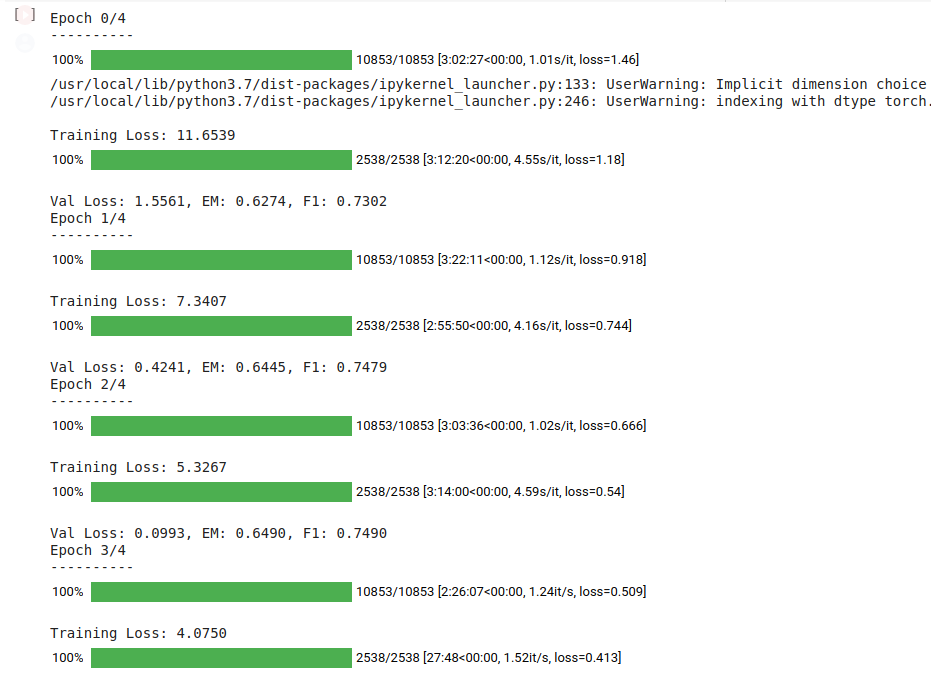
\includegraphics[scale=0.35]{../images/AdamW3e.png}
			\caption{BOLT with AdamW Optimizer at 3e-5 rate}\label{adam3e}
		\end{figure}

		\begin{figure}[!h]
			\centering
			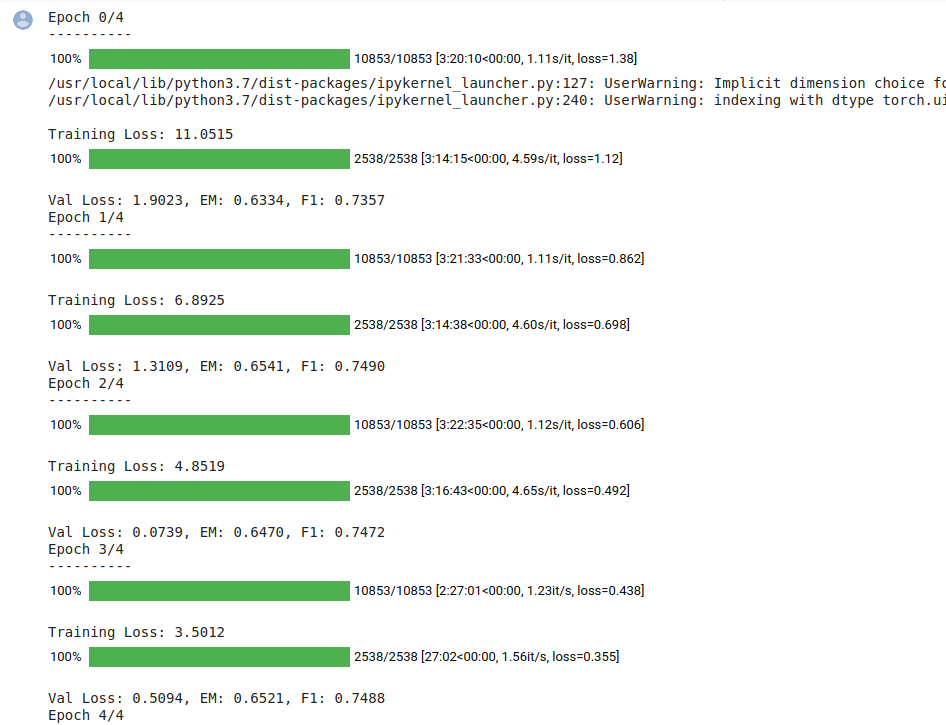
\includegraphics[scale=0.35]{../images/AdaFactor3e.png}
			\caption{BOLT with AdaFactor Optimizer at 3e-5 rate}\label{ada3e}
		\end{figure}

	In the final experiment, that is shown in fig. \ref{ada3e}, the custom model is run with a modified AdaFactor optimizer with a learning rate of 3e-5, this again presents similar results to the results in the previous experiment where the lower value of the learning rate helped the custom model learn better. The training loss for this run also falls similar to the loss in the previous custom model experiments as well as the DistilBERT benchmark, while maintaing an F1 score that is higher than the DistilBERT benchmark but roughly similar to the custom model with AdamW optimizer at a learning rate of 3e-5.


        Figure \ref{ada3e-output} shows the DistilBERT custom model producing correct answers to a few question asked of it. This confirms that the model is able to produce answers to some questions and can give accurate results as well. The custom model is more accurate than its base DistilBERT model, who's output can be seen in figure \ref{distilOut}. While the DistilBERT model answers the first 2 questions correctly, it fails to answer the final question, ``What problem can LSTM suffer from?", with 100\% accuracy and outputs ``vanishing gradient problem" instead of the correct answer ``exploding gradient problem".
		\begin{figure}[!h]
			\centering
			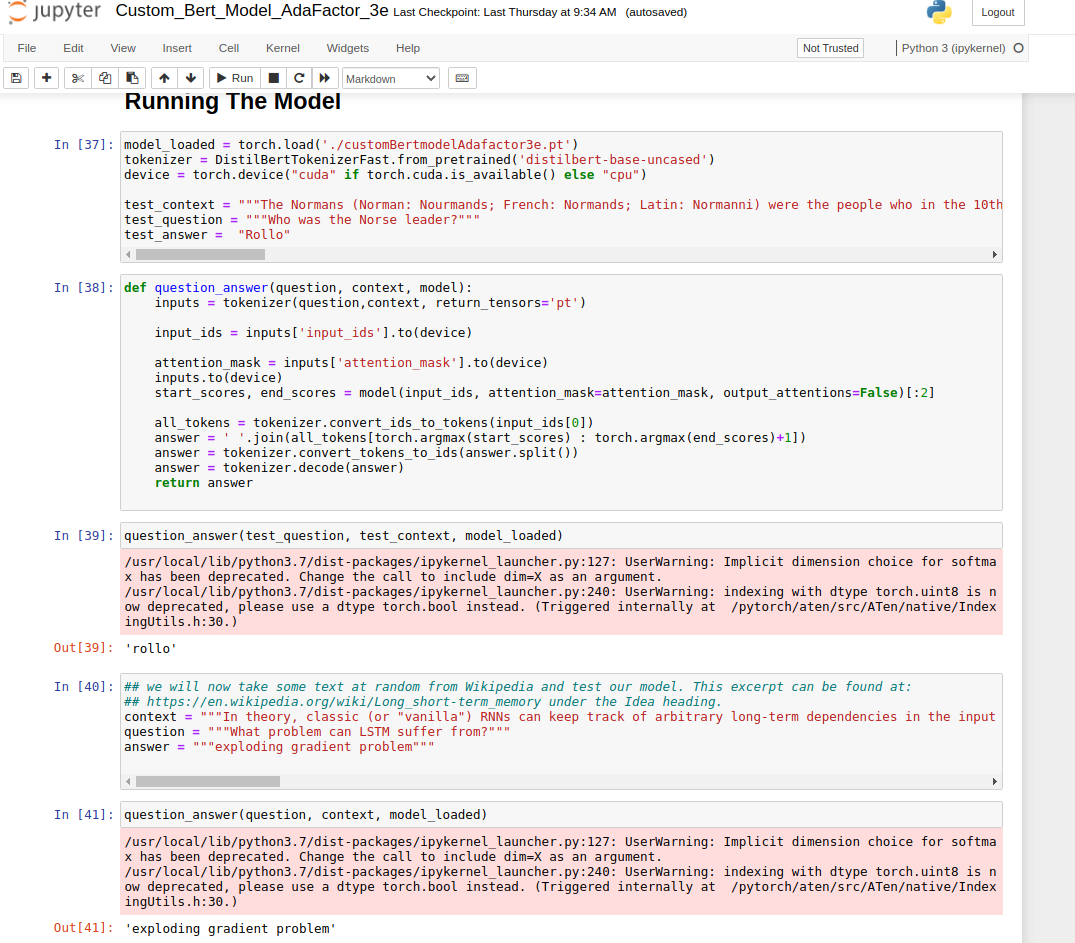
\includegraphics[scale=0.35]{../images/AdaFactor3e-output.png}
			\caption{BOLT with AdaFactor Optimizer at 3e-5 rate outputs to questions asked}\label{ada3e-output}
		\end{figure}
		\begin{figure}[!h]
			\centering
			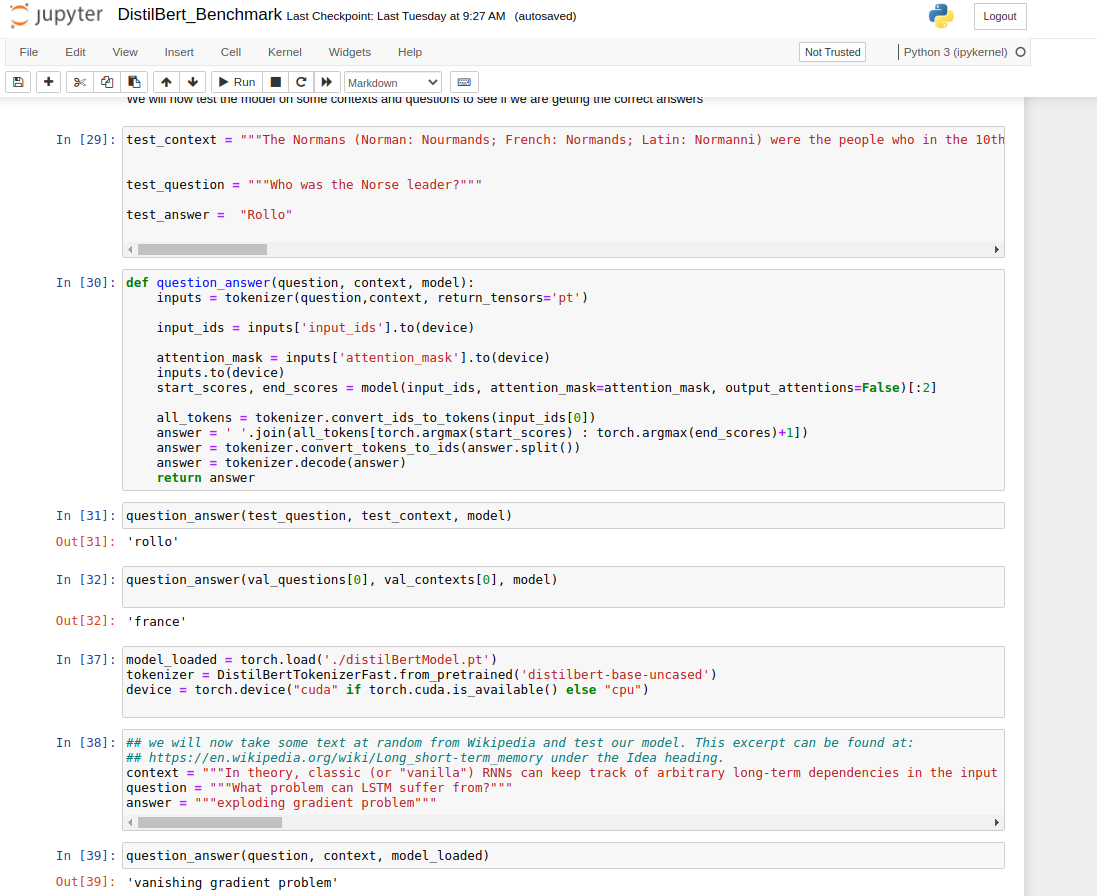
\includegraphics[scale=0.35]{../images/distilbert-answers.png}
			\caption{DistilBERT model outputs to questions asked}\label{distilOut}
		\end{figure}


    \chapter{Conclusions And Recommendations}\label{c6}

    Through this work it has attempted to highlight the advancements and propose a unique modification to the existing transformer architecture using an Answer-Pointer network.

    The results obtained from experiments in section \ref{c52} show that the models performance is at par with the DistilBERT model. While this result isn't graphically present due to timeout issues in Google Colab, visually the various scores printed in figures \ref{adam5e}, \ref{adam3e} and \ref{ada3e}, the model does perform well initially.

    The experiments conducted in this thesis highlight that a properly implemented LSTM based Answer Pointer network layer that is incorporated with the Transformer architecture can perform at par with a current state of the art model.
    While the custom model presents an opportunity for improvement in terms of training times, the results and the metrics are at par with the benchmark models.

    The benchmarked models are current state of the art approaches that are used industry wide for various applications and readily available via libraries like PyTorch, Hugging Face and TensorFlow. The model presented here has shown potential through the limited amount of testing and resources available.

    It is highly probable that given the right resources and time to optimize the model, it will be able to perform better than the DistilBERT model at least.

    \section{Recommendations}

    This work provides a unique opportunity to introduce improvements to an already state of the art architecture by adding a layer of LSTM based pointers. Highlighted below are some recommendations that can improve the architecture further.

    \begin{itemize}

    	\item \textbf{Training Checkpoints}: Checkpointing and training the models across various checkpoints can help run the model for more number of epochs by saving and resuming trainging from a particular checkpoint. This is especially critical in the case of using online resources such as Google Colab because they disconnect runtimes after 24 hours and wipe all the data.

    	\item \textbf{Increased Batch-Size}: The experiments presented in this work are limited by a relatively small batch size of 8. Systemic increase of batch size can allow for reduced training times, possibly better performance overall and an opportunity to test this model against various other NLP applications such as Sequence Classification, Token Classification, Sentence Predictions, etc.

    	\item \textbf{Better Hardware}: One of the key limiting factors for the work presented in this thesis is the limiting amount of VRAM, The current hardware used only had 8GB of VRAM available on the EVGA 2070 Super GPU, which was insufficient for the benchmark batch size of 8. Reducing the batch size any further led to increased training times per epoch, upwards of 3 hours per epoch at a batch size of 6. This problem was slightly remediated by the use of Google Colab Pro, which is a subscriptions service that allows you to run experiments using better GPUs such as Tesla P100 GPU with 16GB VRAM. This service is time limited and thus not suitable for running long experiments. To effectively quantify the proposed architecture in this thesis it is recommended that it be run for at least 10 epochs on a multi-GPU setup that allows for mini-batches. This approach is discussed below.

    	\item \textbf{Mini-Batches Across Multiple GPUs}: Creating a multi-GPU setup, with 2 or more gpus, allows for accelerated training \citep{multigpu1}. A simple guide on how to set this up for PyTorch has been created on the Towards Data Science Medium page \citep{multigpu2}. Having multiple smaller batches train across a multi-GPU setup can allow the model to not only train faster but also perfrom slightly better than just on a single GPU.

    	\item \textbf{Increased LSTM Model Complexity}: One of the biggest challenges faced was increasing model complexity from implementing a single LSTM model with 8 hidden layers to anything more or even bidirectional in nature. The experiments conducted using more number of LSTM layers or hidden layers led to very high GPU memory usage, often causing out of memory errors, hence failing model training. If the above recommendations are provided then it might be possible to increase the LSTM model complexity which could yeild better F1 and Exact Match scores for predictions by the model.
    \end{itemize}

   \begin{appendices}
    	\chapter{Gantt Chart}\label{cgc}
		    \begin{figure}[!h]
		       	\centering
		        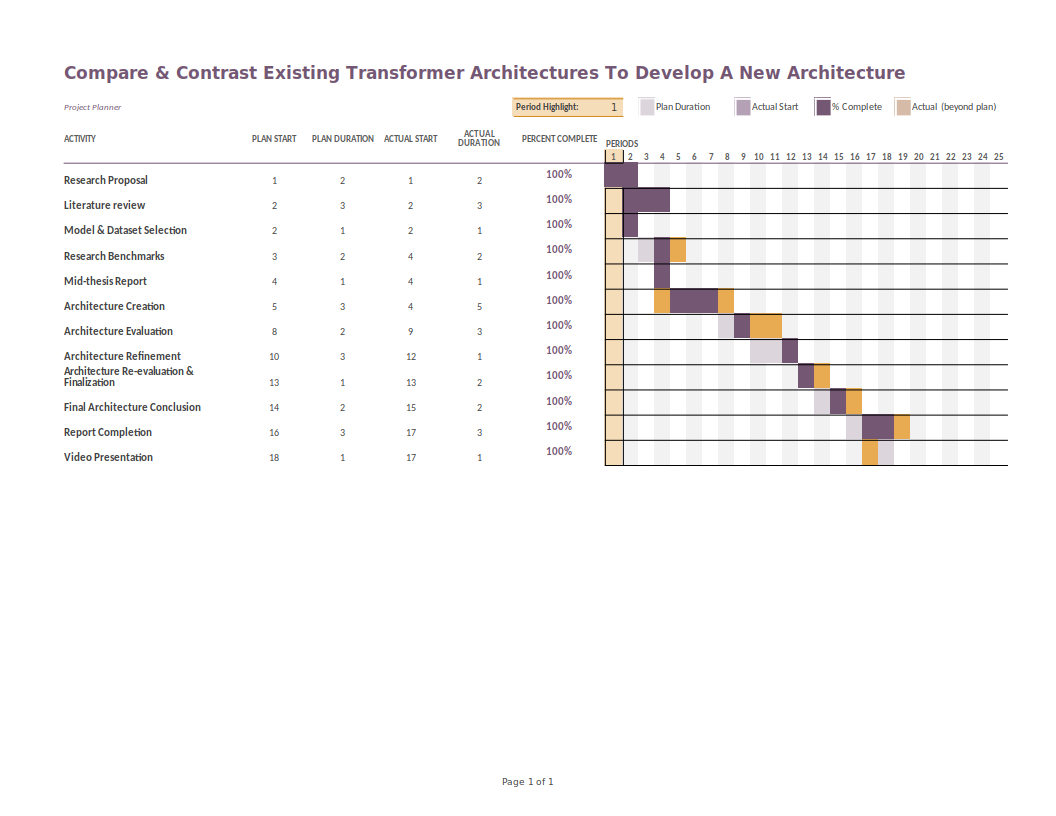
\includegraphics[scale=0.55,angle=90]{../images/GanttChart-final.png}
		     	\caption{Thesis Gantt Chart}\label{ganttChartMid}
              \end{figure}
         \chapter{Research Proposal}\label{crp}
         	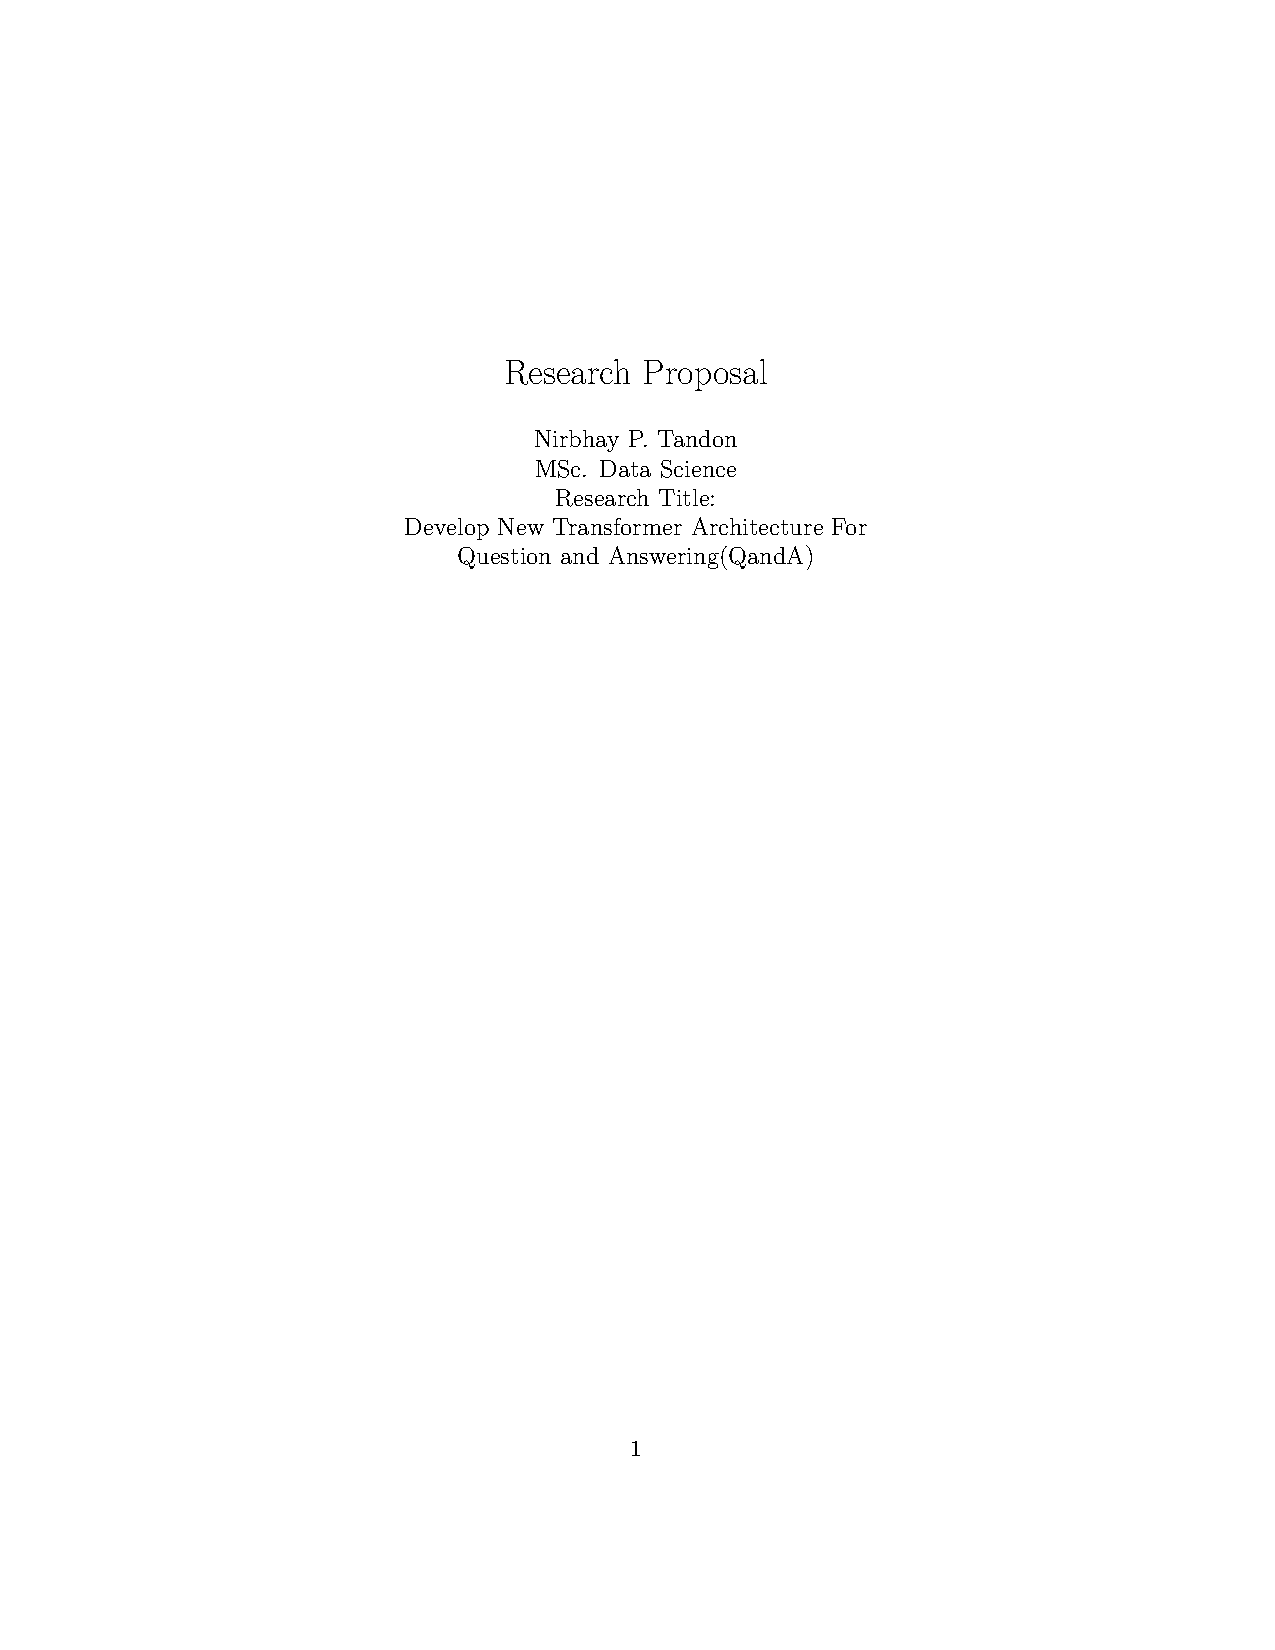
\includepdf[pages=1-15]{../rp.pdf}

    \end{appendices}


%\setcitestyle{numbers}
%\nocite{*}
\bibliography{FinalThesis}
\end{document}